\documentclass[conference]{IEEEtran}

\usepackage{cite}
\usepackage{amsmath,amssymb,amsfonts}
\usepackage{algorithmic}
\usepackage{graphicx}
\usepackage{textcomp}
\usepackage{xcolor}
\usepackage{gensymb}
\usepackage{tikz}
\usepackage{float}
\usepackage{hyperref}
\usepackage{enumerate}
\usepackage{subcaption}
\def\BibTeX{{\rm B\kern-.05em{\sc i\kern-.025em b}\kern-.08em
    T\kern-.1667em\lower.7ex\hbox{E}\kern-.125emX}}
\begin{document}

\title{4-bit CLA Adder \\ VLSI Course Project}

\author{\IEEEauthorblockN{1\textsuperscript{st} Vignesh Vembar}
\IEEEauthorblockA{\textit{ECE, IIIT Hyderabad} \\
\textit{2023102019}\\
vigneshvembar.m@students.iiit.ac.in}
}

\maketitle

\begin{abstract}
This document is a report on the Design and Simulation of a 4-bit Carry Look Ahead Adder.
\end{abstract}


\section{Introduction}
The Carry Look Ahead Adder is a digital circuit that is used to add two 4 bit binary numbers. It is faster than the Ripple Carry Adder as it generates the carry signals for all the bits at the same time. 

\section{Proposed Design}

\subsection{CLA Adder}

\subsection{D Flip Flop}

\section{Verilog Simulation}

\subsection{CLA Adder}

\begin{figure}[H]
    \centering
    \includegraphics[width=0.48\textwidth]{images/verilog_cla.png}
    \caption{GTKWave Plot of CLA Adder Verilog Simulation}
\end{figure}

\subsection{D Flip Flop}

\begin{figure}[H]
    \centering
    \includegraphics[width=0.48\textwidth]{images/verilog_d_ff.png}
    \caption{GTKWave Plot of  D Flip Flop Verilog Simulation}
\end{figure}
\subsection{Full Circuit}

\section{NGSPICE Simulation}

\subsection{Inverter}

\begin{figure}[H]
    \centering
    \includegraphics[width=0.48\textwidth]{images/inv_cmos_tran.eps}
    \caption{NGSPICE Plot of Inverter}
\end{figure}

\subsection{NAND Gate}

\begin{figure}[H]
    \centering
    \begin{tabular}{cc}
        \begin{subfigure}{0.44\linewidth}
            \centering
            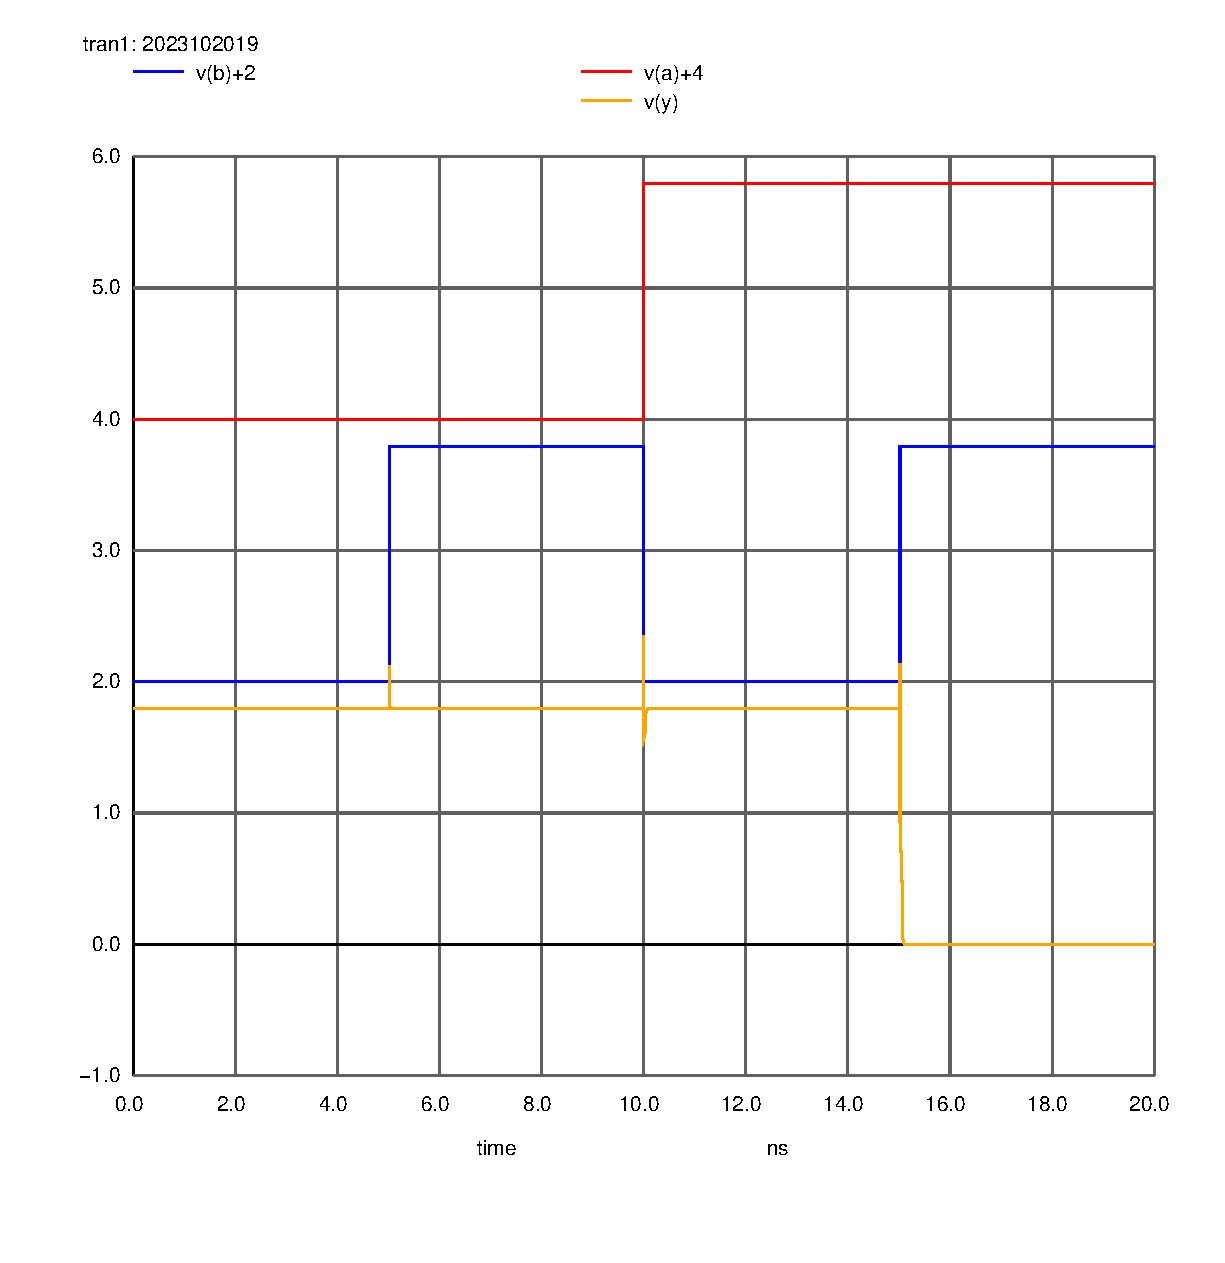
\includegraphics[width=\textwidth]{images/nand_cmos_tran.eps}
            \caption{2 Input NAND}
        \end{subfigure} &
        \begin{subfigure}{0.44\linewidth}
            \centering
            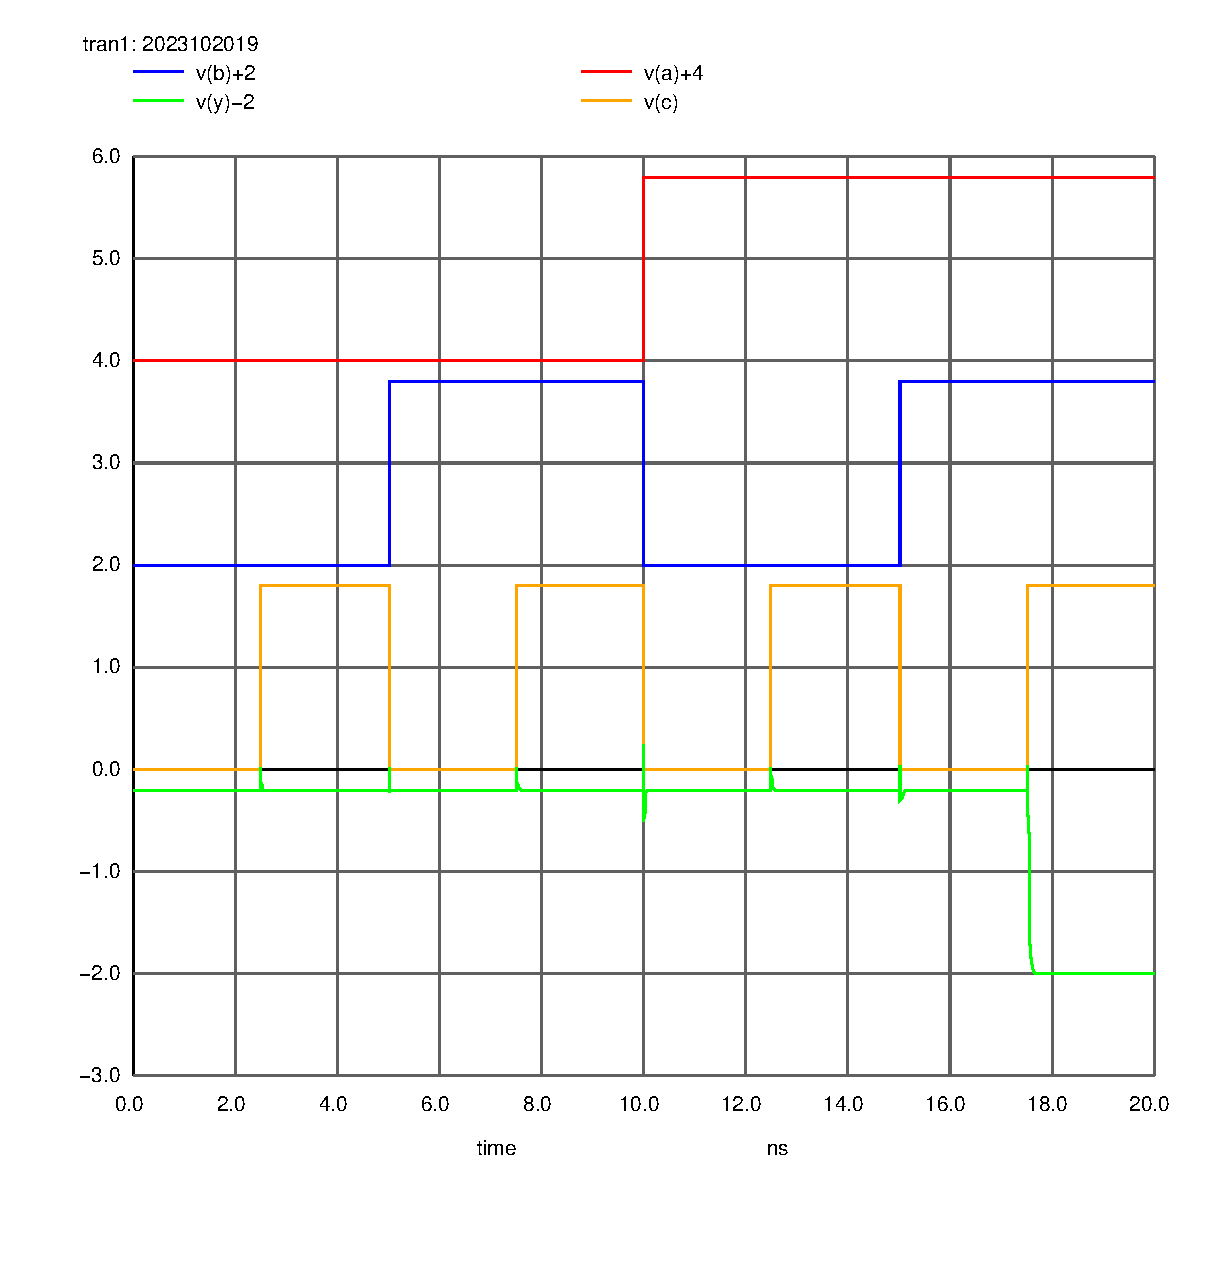
\includegraphics[width=\textwidth]{images/nand_3_cmos_tran.eps}
            \caption{3 Input NAND}
        \end{subfigure} \\
        \begin{subfigure}{0.44\linewidth}
            \centering
            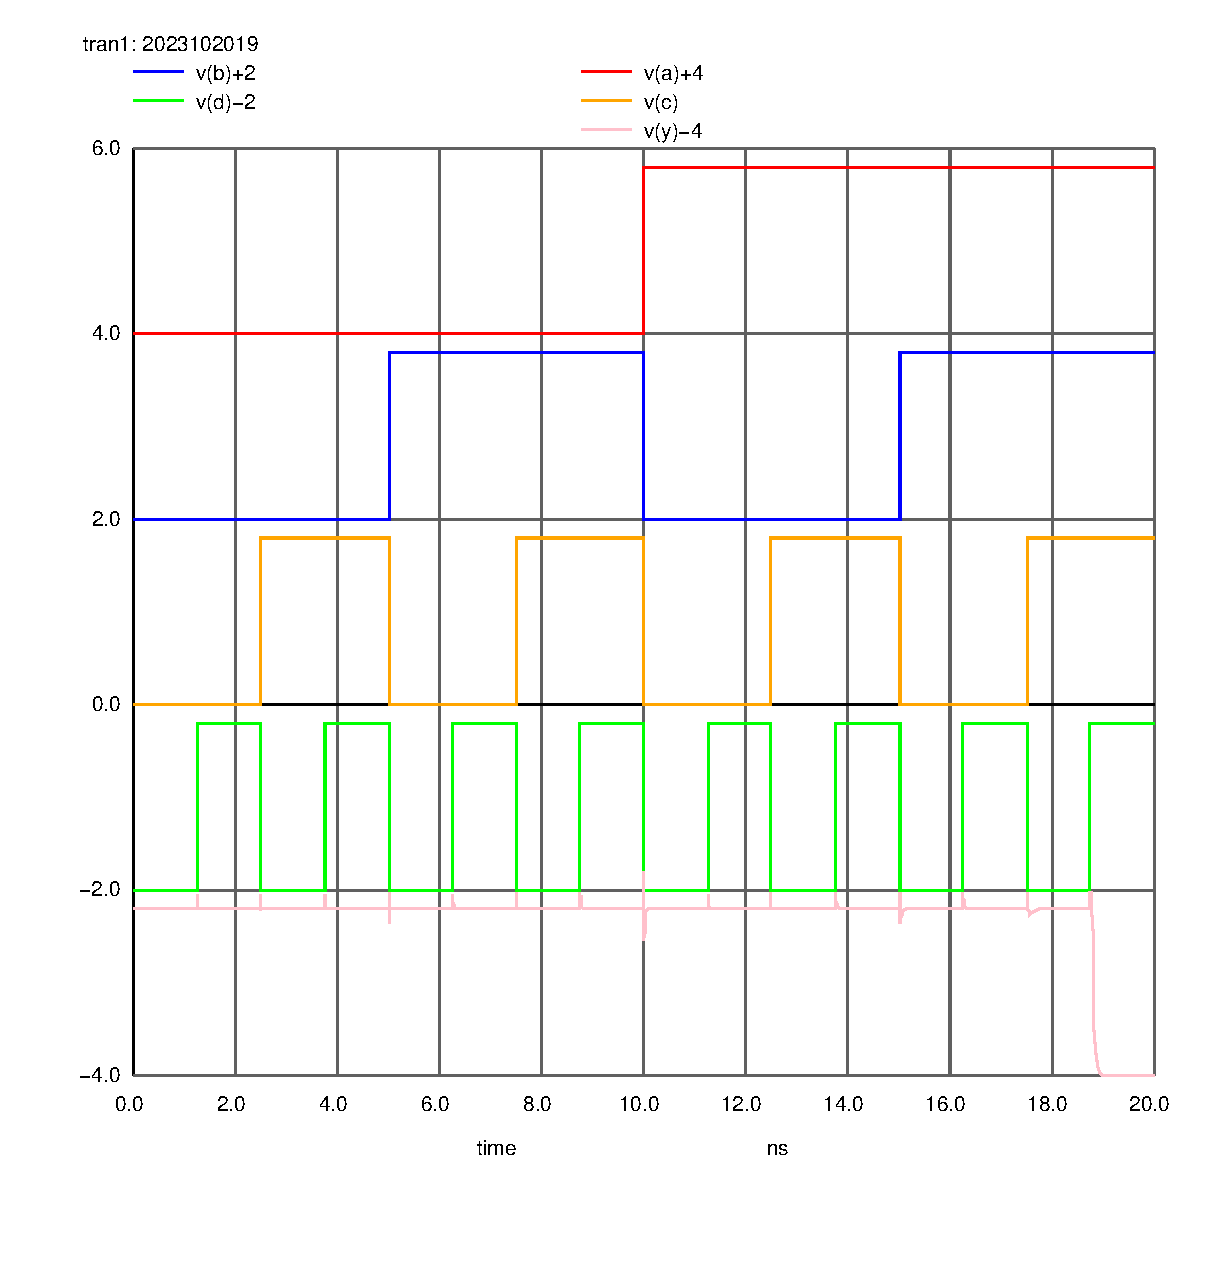
\includegraphics[width=\textwidth]{images/nand_4_cmos_tran.eps}
            \caption{4 Input NAND}
        \end{subfigure} &
        \begin{subfigure}{0.44\linewidth}
            \centering
            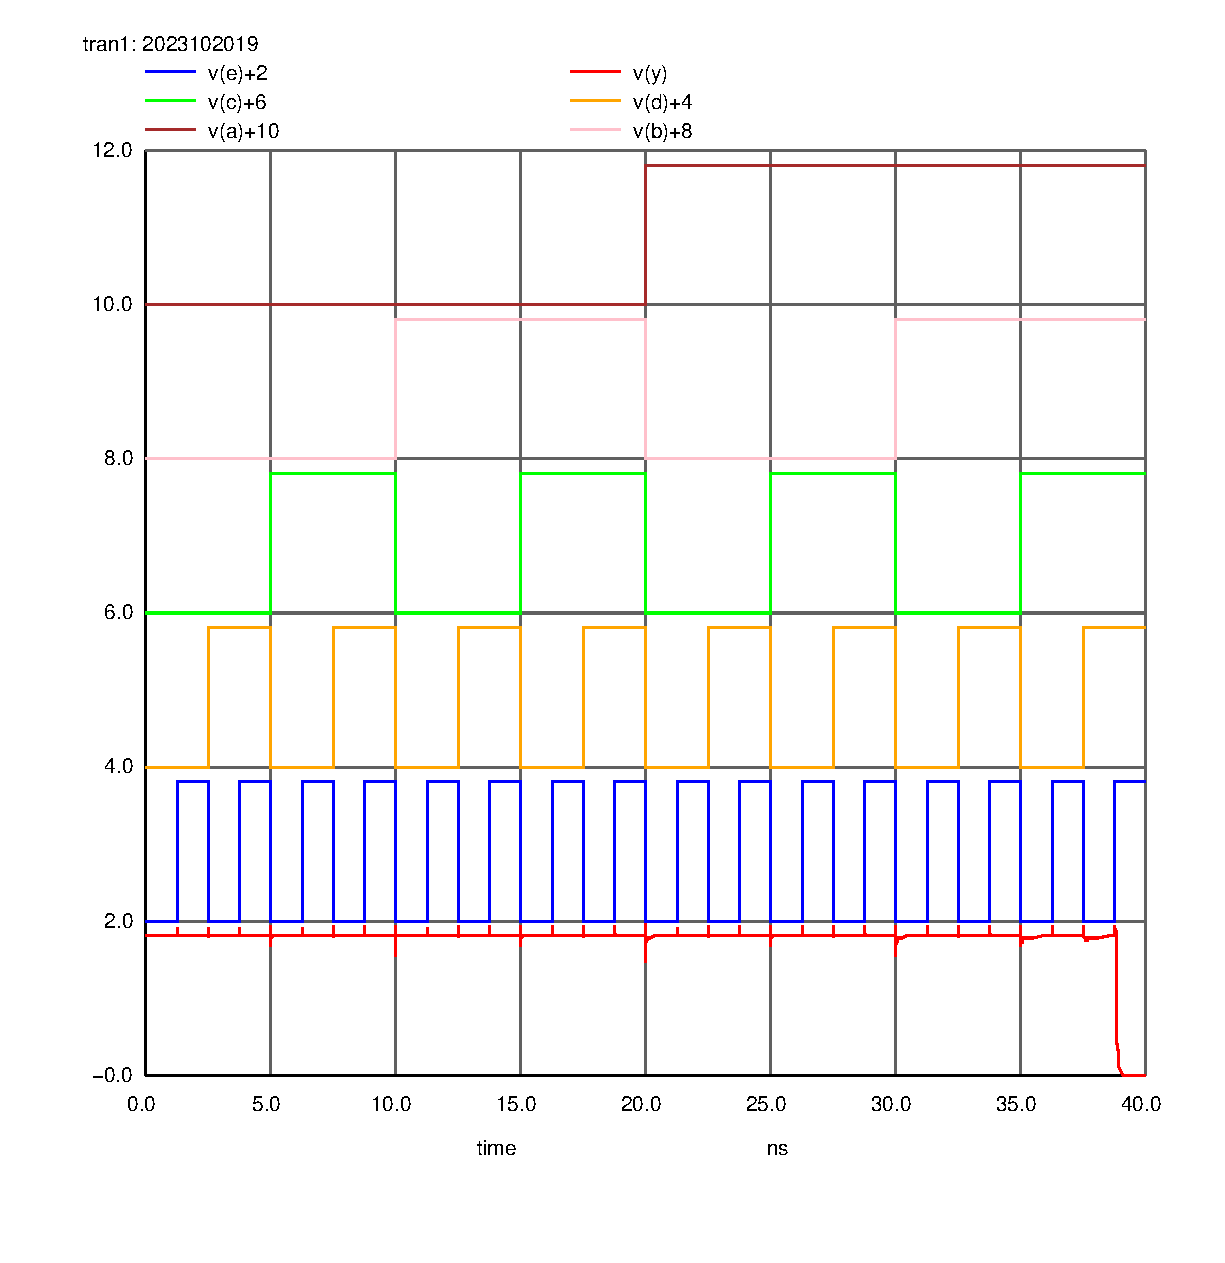
\includegraphics[width=\textwidth]{images/nand_5_cmos_tran.eps}
            \caption{5 Input NAND}
        \end{subfigure}
    \end{tabular}
    \caption{NGSPICE Plot of NAND Gates}
\end{figure}

\subsection{NOR Gate}

\begin{figure}[H]
    \centering
    \begin{tabular}{cc}
        \begin{subfigure}{0.44\linewidth}
            \centering
            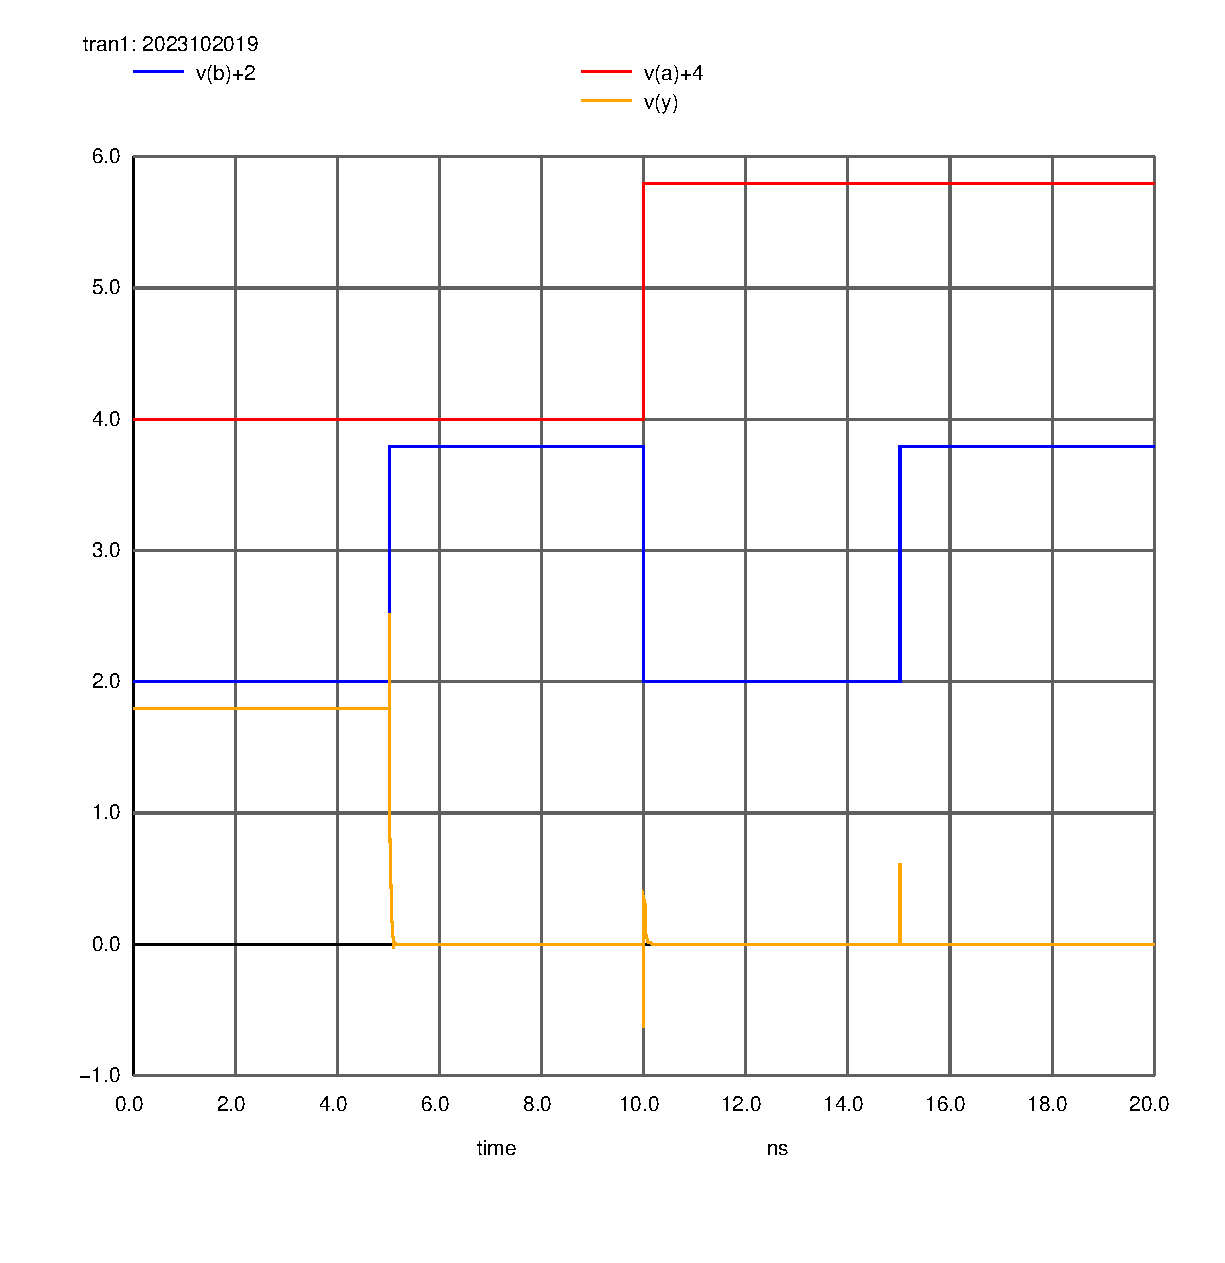
\includegraphics[width=\textwidth]{images/nor_cmos_tran.eps}
            \caption{2 Input NOR}
        \end{subfigure} &
        \begin{subfigure}{0.44\linewidth}
            \centering
            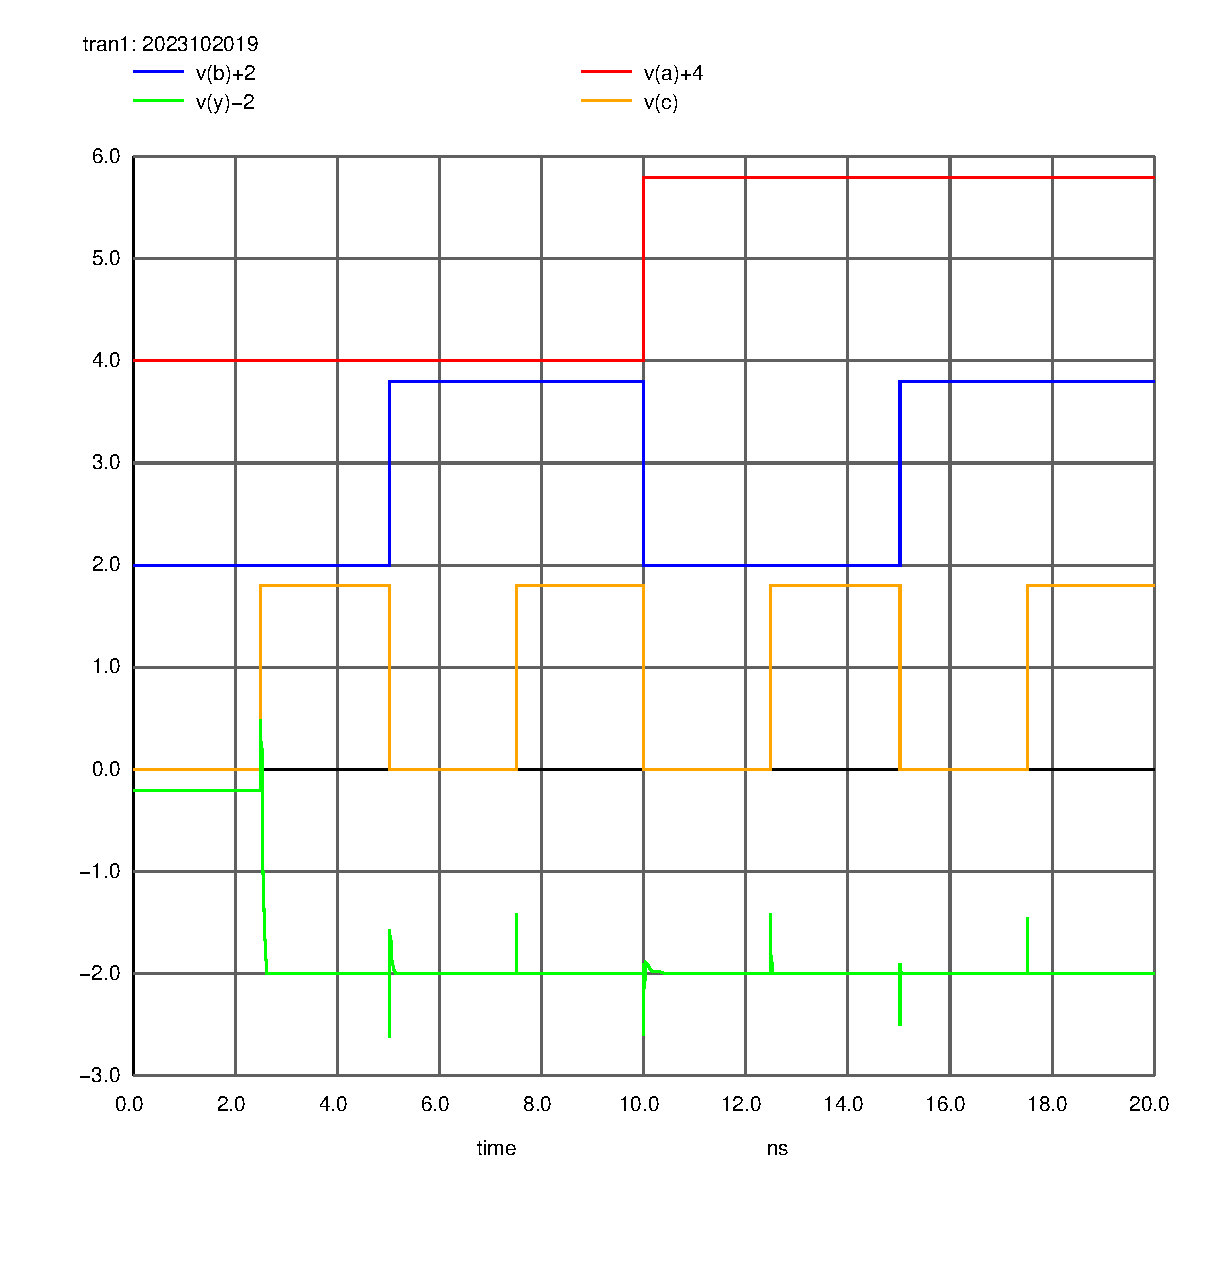
\includegraphics[width=\textwidth]{images/nor_3_cmos_tran.eps}
            \caption{3 Input NOR}
        \end{subfigure} \\
        \begin{subfigure}{0.44\linewidth}
            \centering
            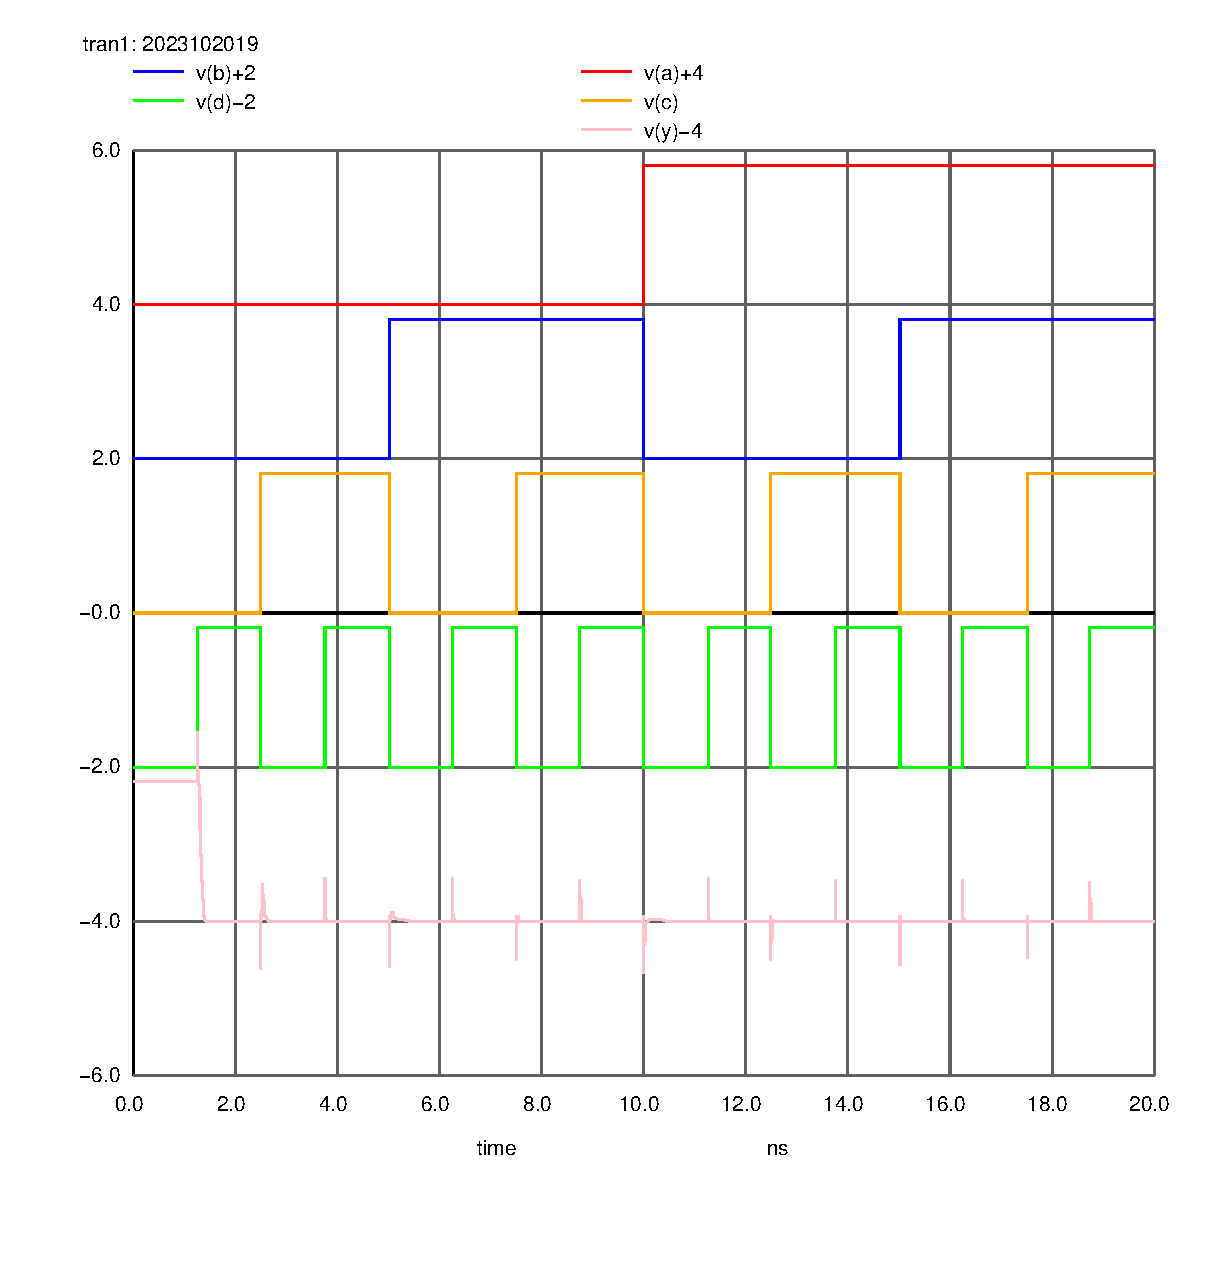
\includegraphics[width=\textwidth]{images/nor_4_cmos_tran.eps}
            \caption{4 Input NOR}
        \end{subfigure} &
        \begin{subfigure}{0.44\linewidth}
            \centering
            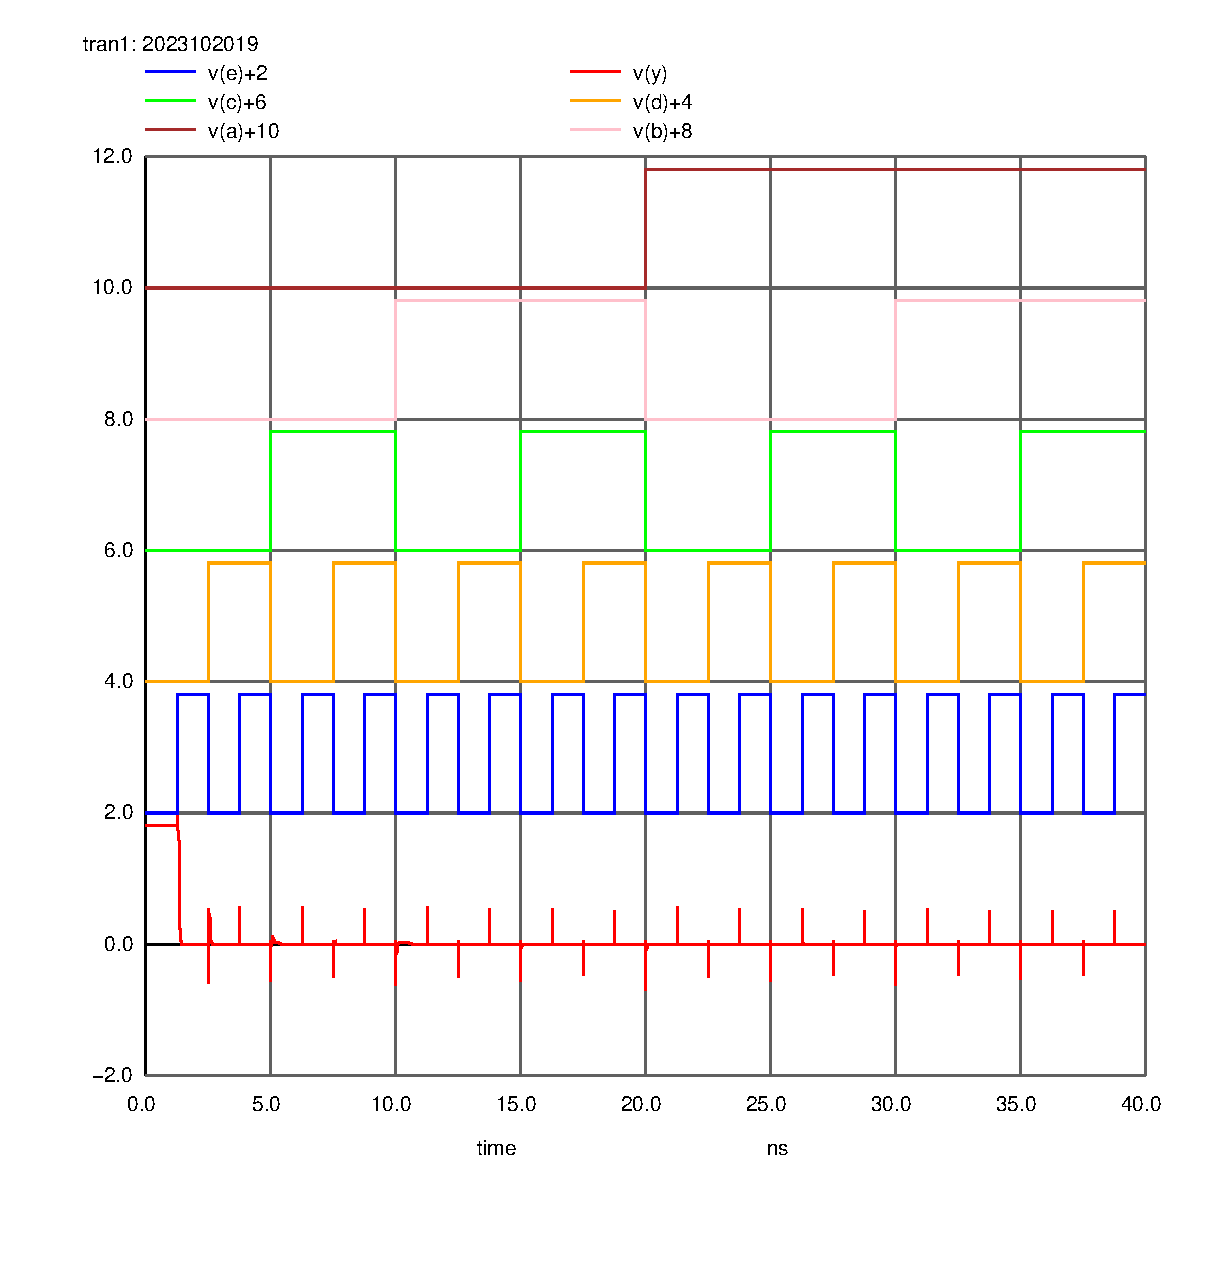
\includegraphics[width=\textwidth]{images/nor_5_cmos_tran.eps}
            \caption{5 Input NOR}
        \end{subfigure}
    \end{tabular}
    \caption{NGSPICE Plot of NOR Gates}
\end{figure}

\subsection{XOR Gate}

\subsubsection{CMOS Implementation}

\begin{figure}[H]
    \centering
    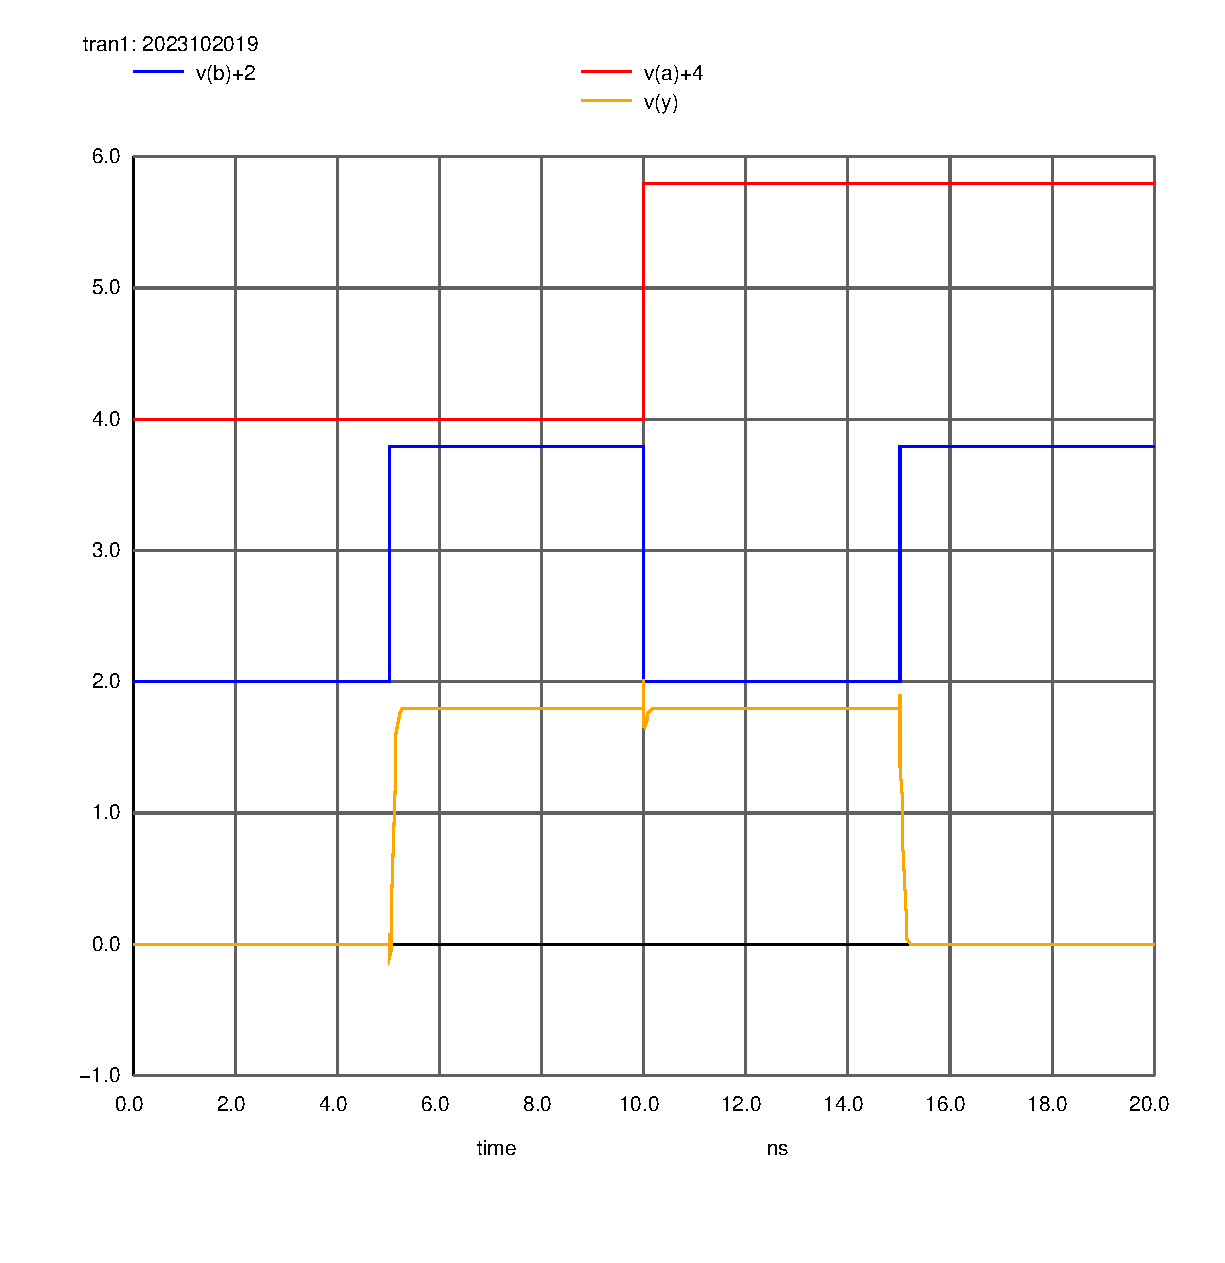
\includegraphics[width=0.48\textwidth]{images/xor_cmos_tran.eps}
    \caption{NGSPICE Plot of CMOS XOR Gate}
\end{figure}

\subsubsection{Complimentary Pass Transistor Implementation}

\begin{figure}[H]
    \centering
    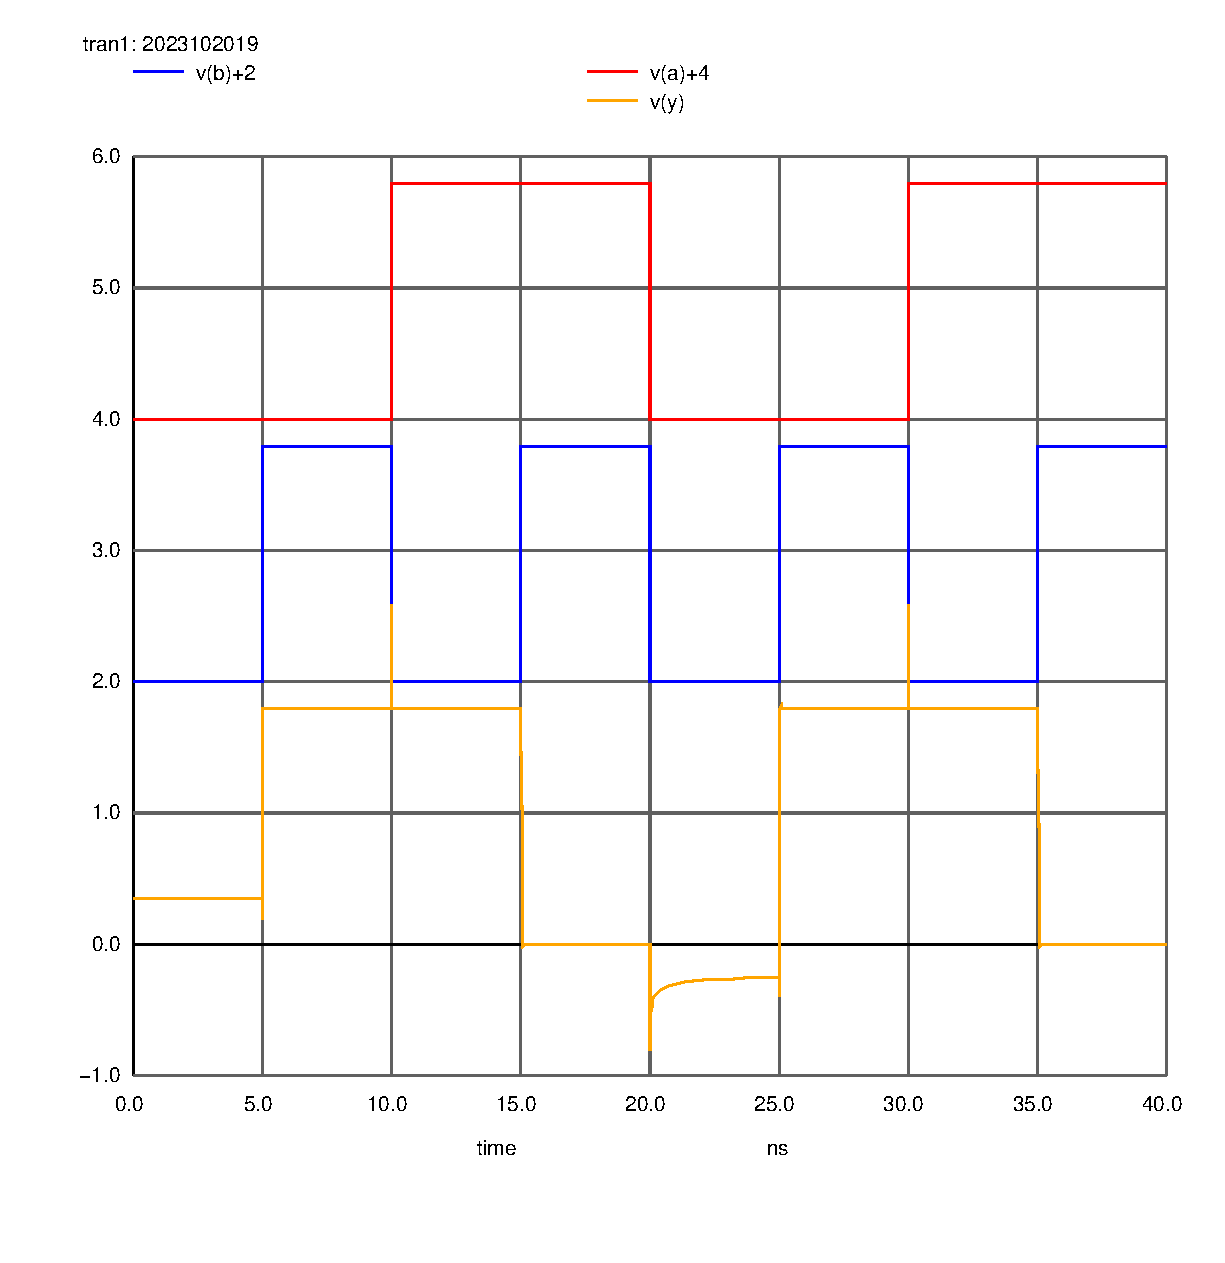
\includegraphics[width=0.48\textwidth]{images/xor_optimized_tran.eps}
    \caption{NGSPICE Plot of CPTL XOR Gate}
\end{figure}

\subsection{Propagate/Generate Generator}

\subsubsection{CMOS Implementation}

\begin{figure}[H]
    \centering
    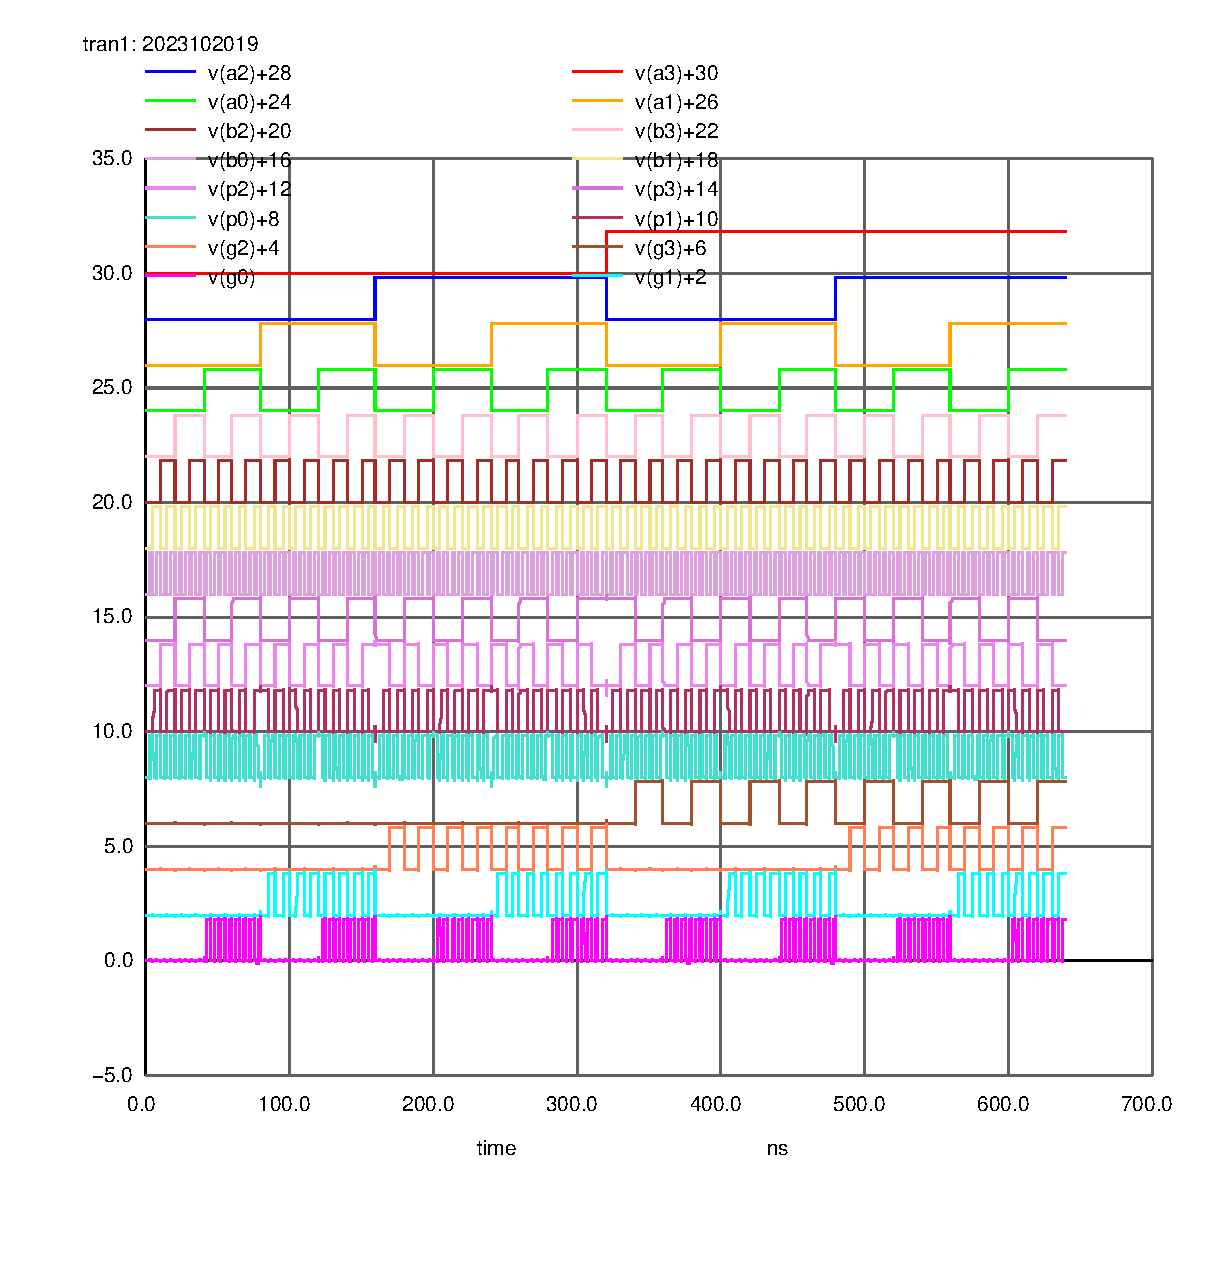
\includegraphics[width=0.48\textwidth]{images/pg_gen_cmos_tran.eps}
    \caption{NGSPICE Plot of CMOS Propagate/Generate Generator}
\end{figure}

\subsubsection{Complimentary Pass Transistor Implementation}

\begin{figure}[H]
    \centering
    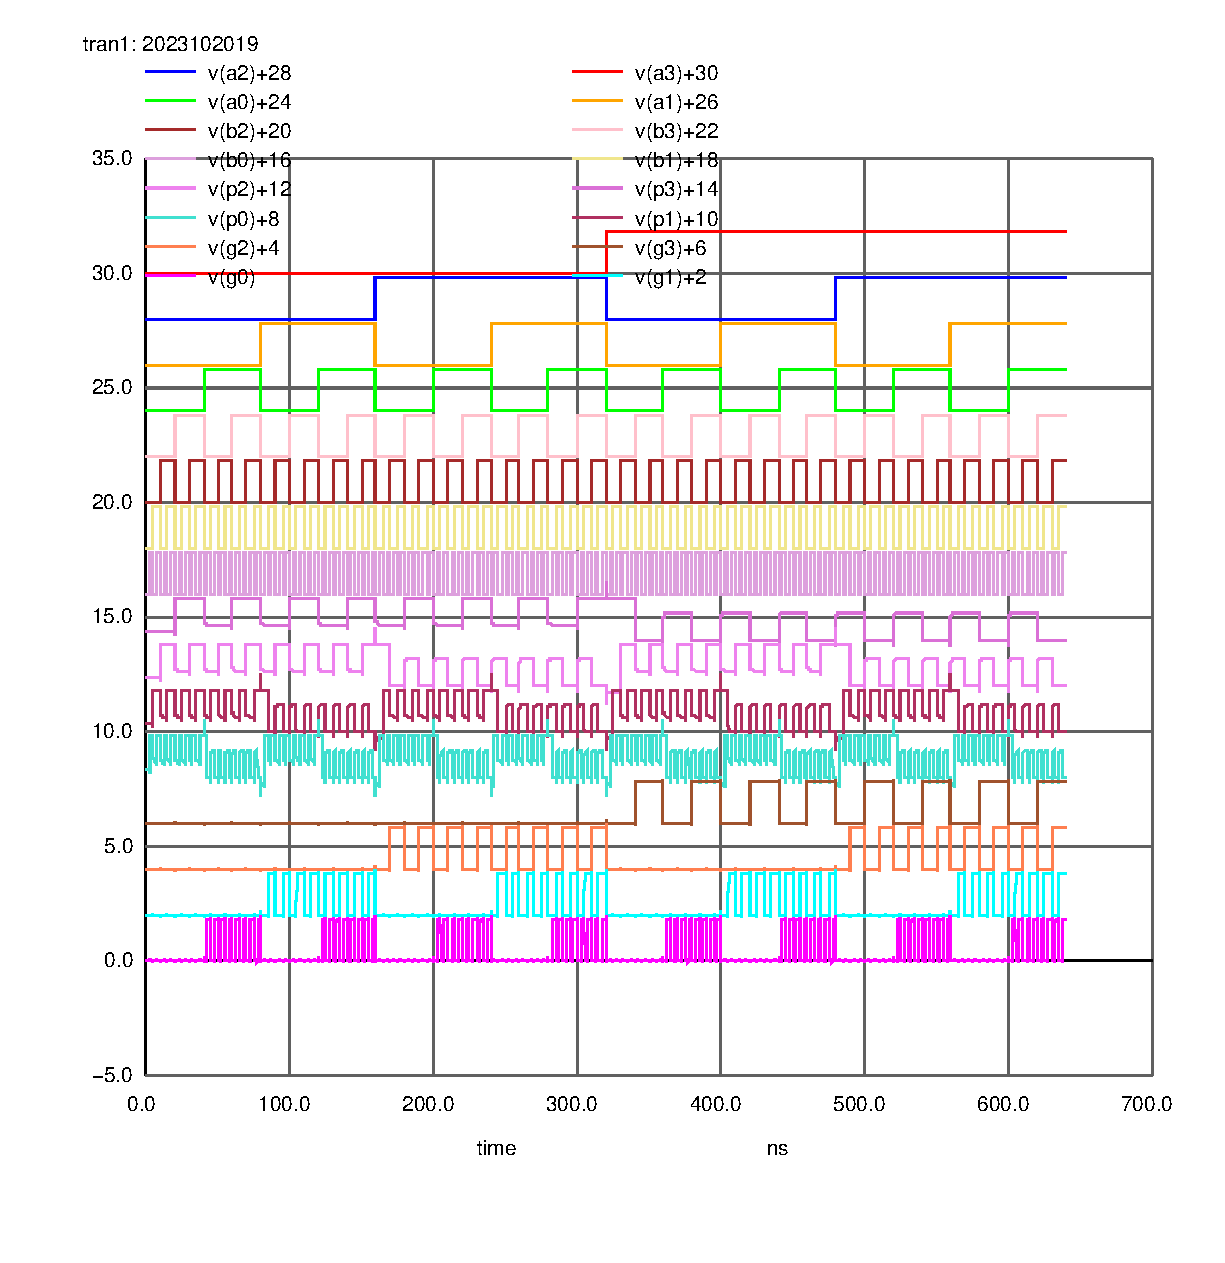
\includegraphics[width=0.48\textwidth]{images/pg_gen_optimized_tran.eps}
    \caption{NGSPICE Plot of CPTL Propagate/Generate Generator}
\end{figure}

\subsection{Carry Look Ahead Generator}

\begin{figure}[H]
    \centering
    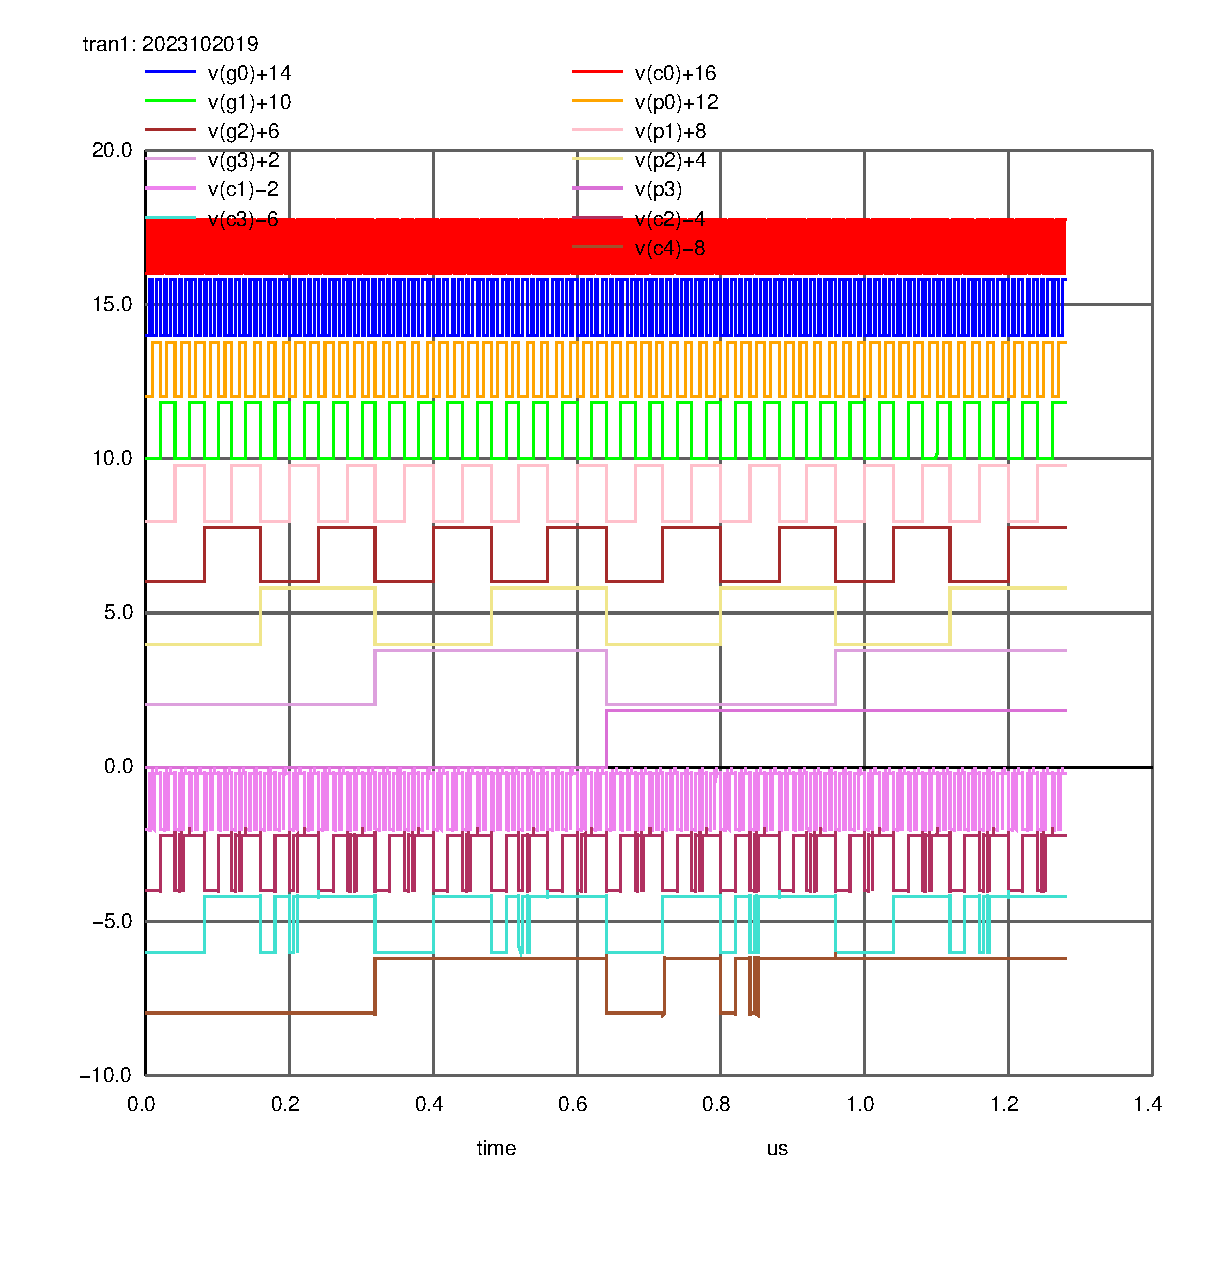
\includegraphics[width=0.48\textwidth]{images/cla_gen_cmos_tran.eps}
    \caption{NGSPICE Plot of CMOS Carry Look Ahead Generator}
\end{figure}

\subsection{Sum Generator}

\subsubsection{CMOS Implementation}

\begin{figure}[H]
    \centering
    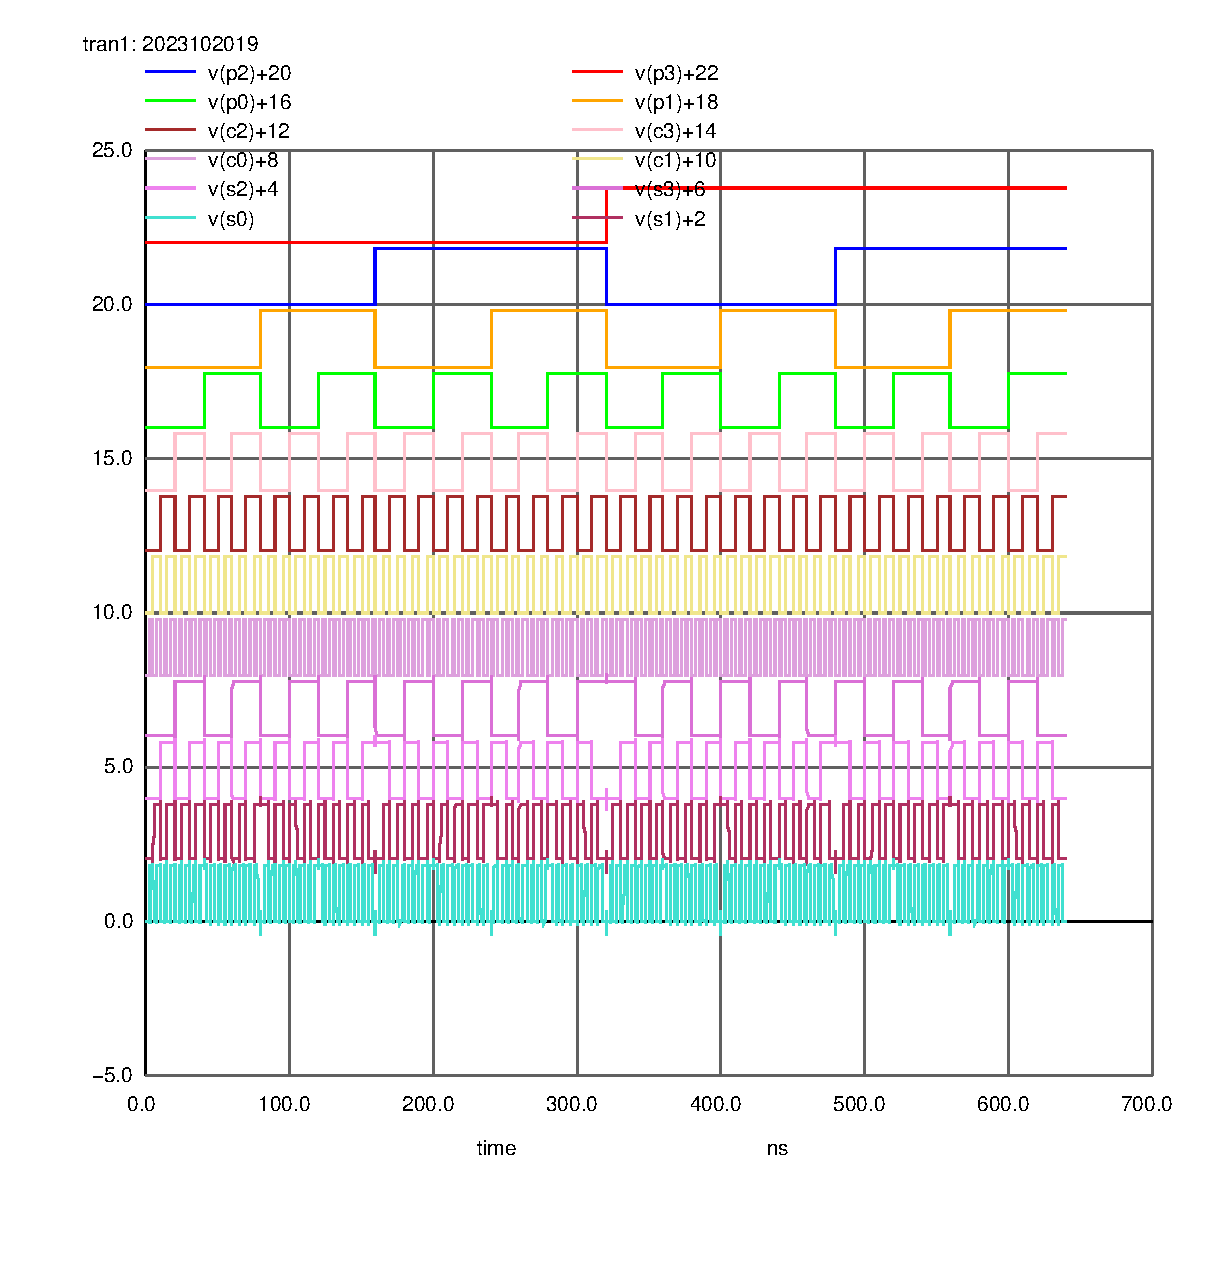
\includegraphics[width=0.48\textwidth]{images/sum_gen_cmos_tran.eps}
    \caption{NGSPICE Plot of CMOS Sum Generator}
\end{figure}

\subsubsection{Complimentary Pass Transistor Implementation}

\begin{figure}[H]
    \centering
    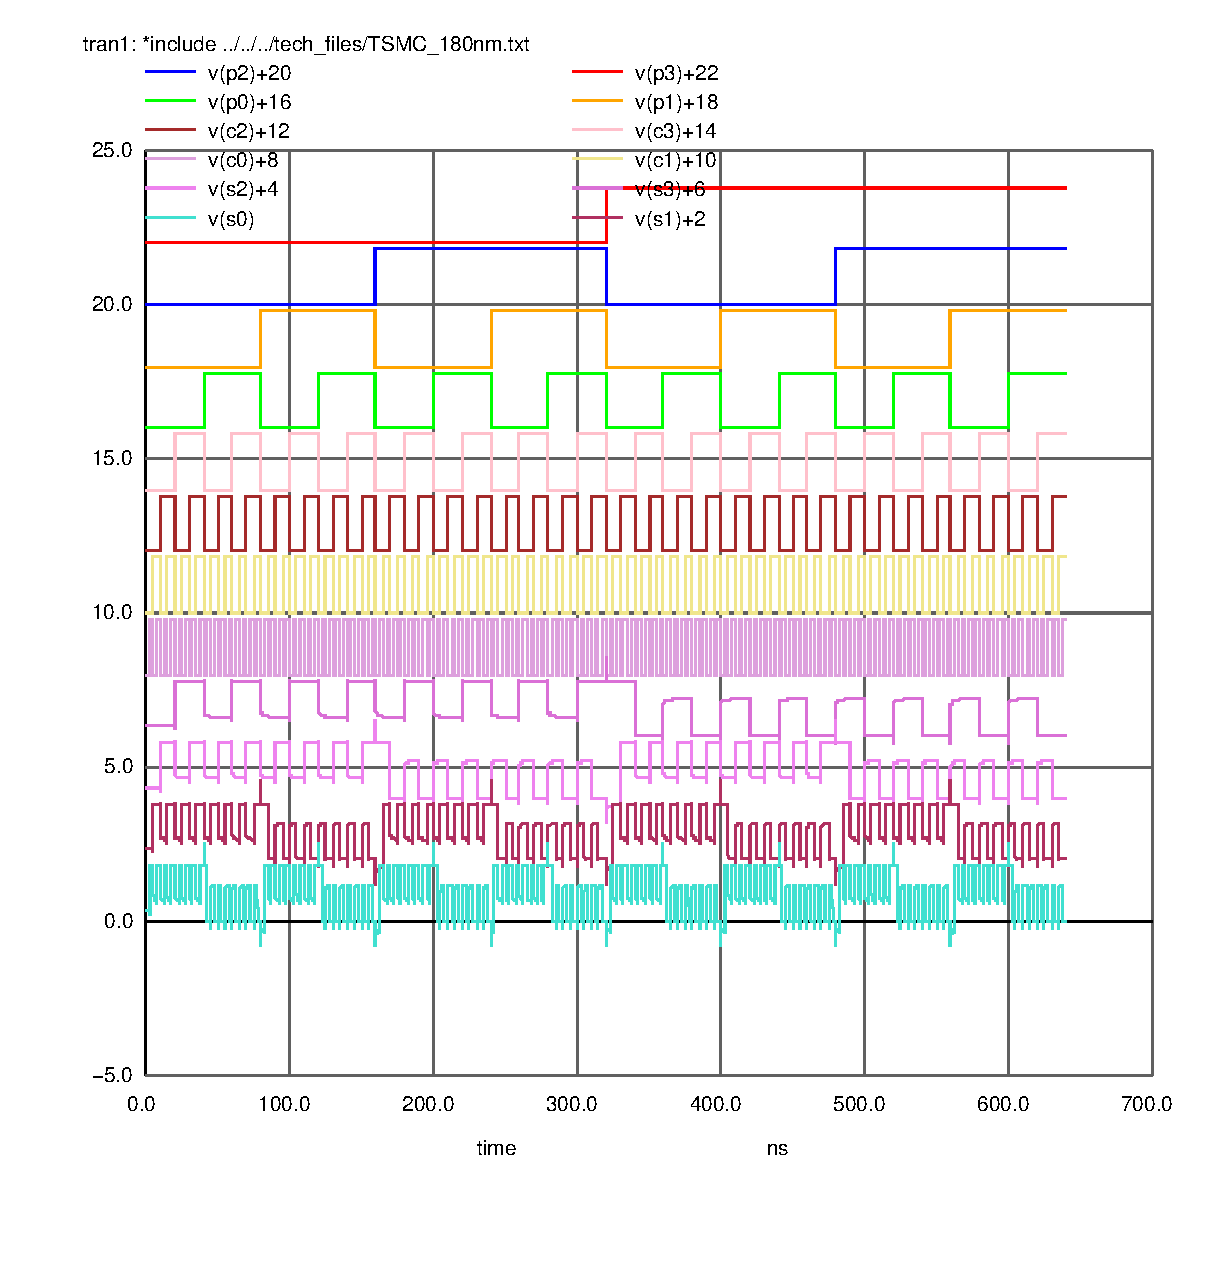
\includegraphics[width=0.48\textwidth]{images/sum_gen_optimized_tran.eps}
    \caption{NGSPICE Plot of CPTL Sum Generator}
\end{figure}

\subsection{D Flop Flop}

\subsubsection{CMOS Implementation}

\begin{figure}[H]
    \centering
    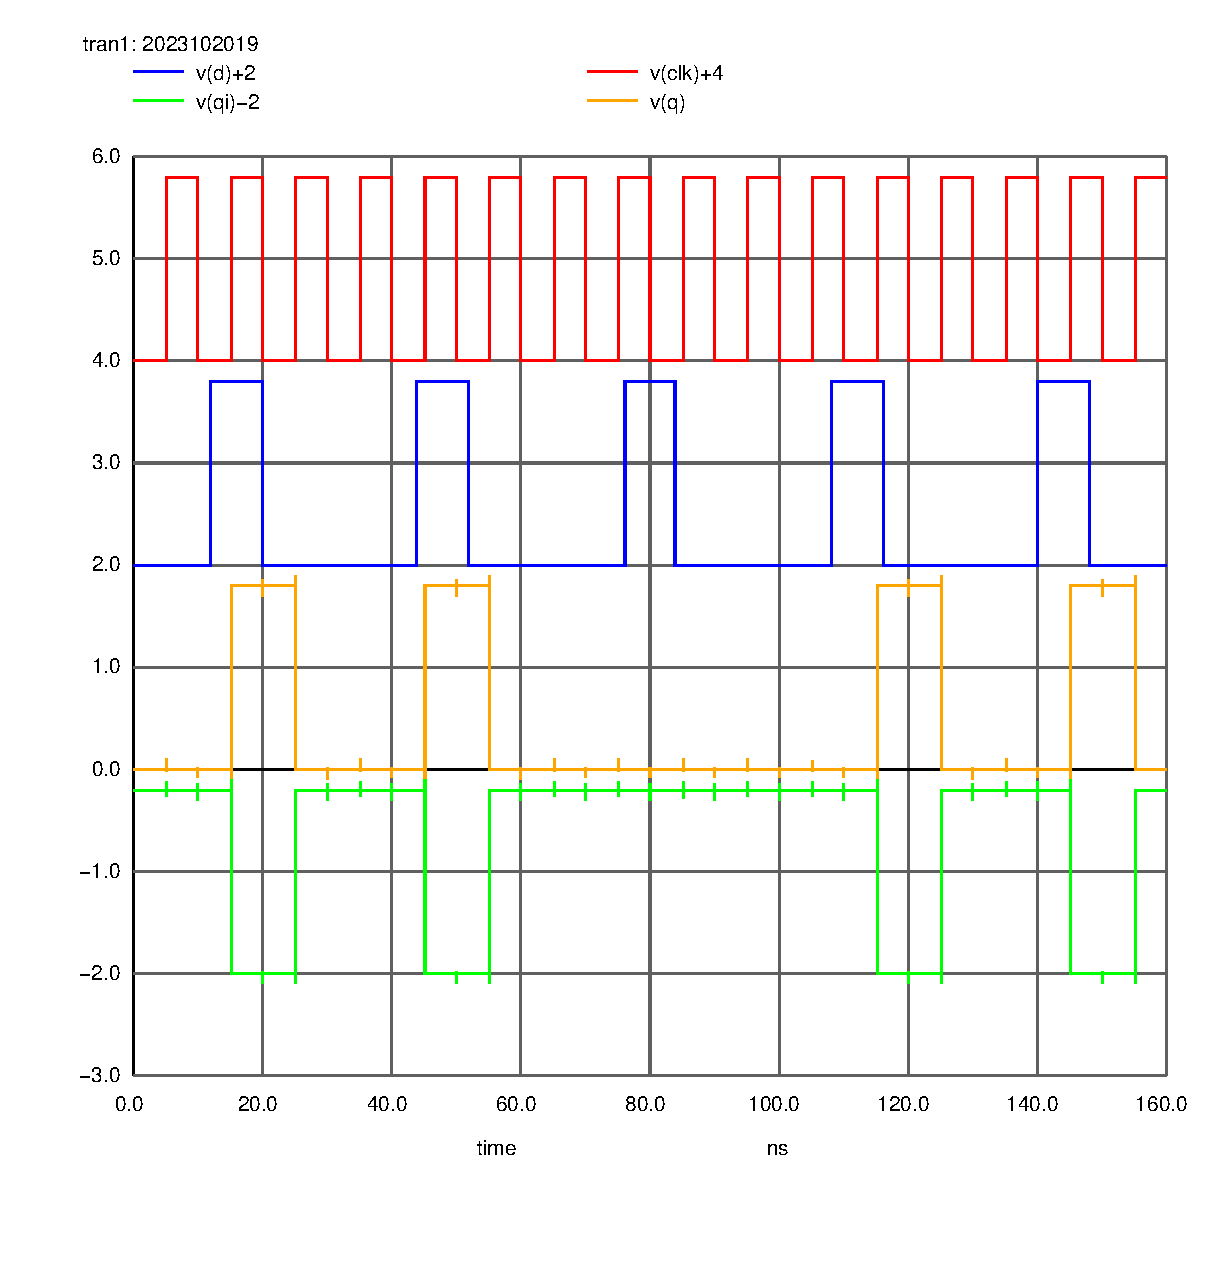
\includegraphics[width=0.48\textwidth]{images/d_ff_cmos_tran.eps}
    \caption{NGSPICE Plot of CMOS D Flip FLop}
\end{figure}

\subsubsection{Optimized Implementation}

\begin{figure}[H]
    \centering
    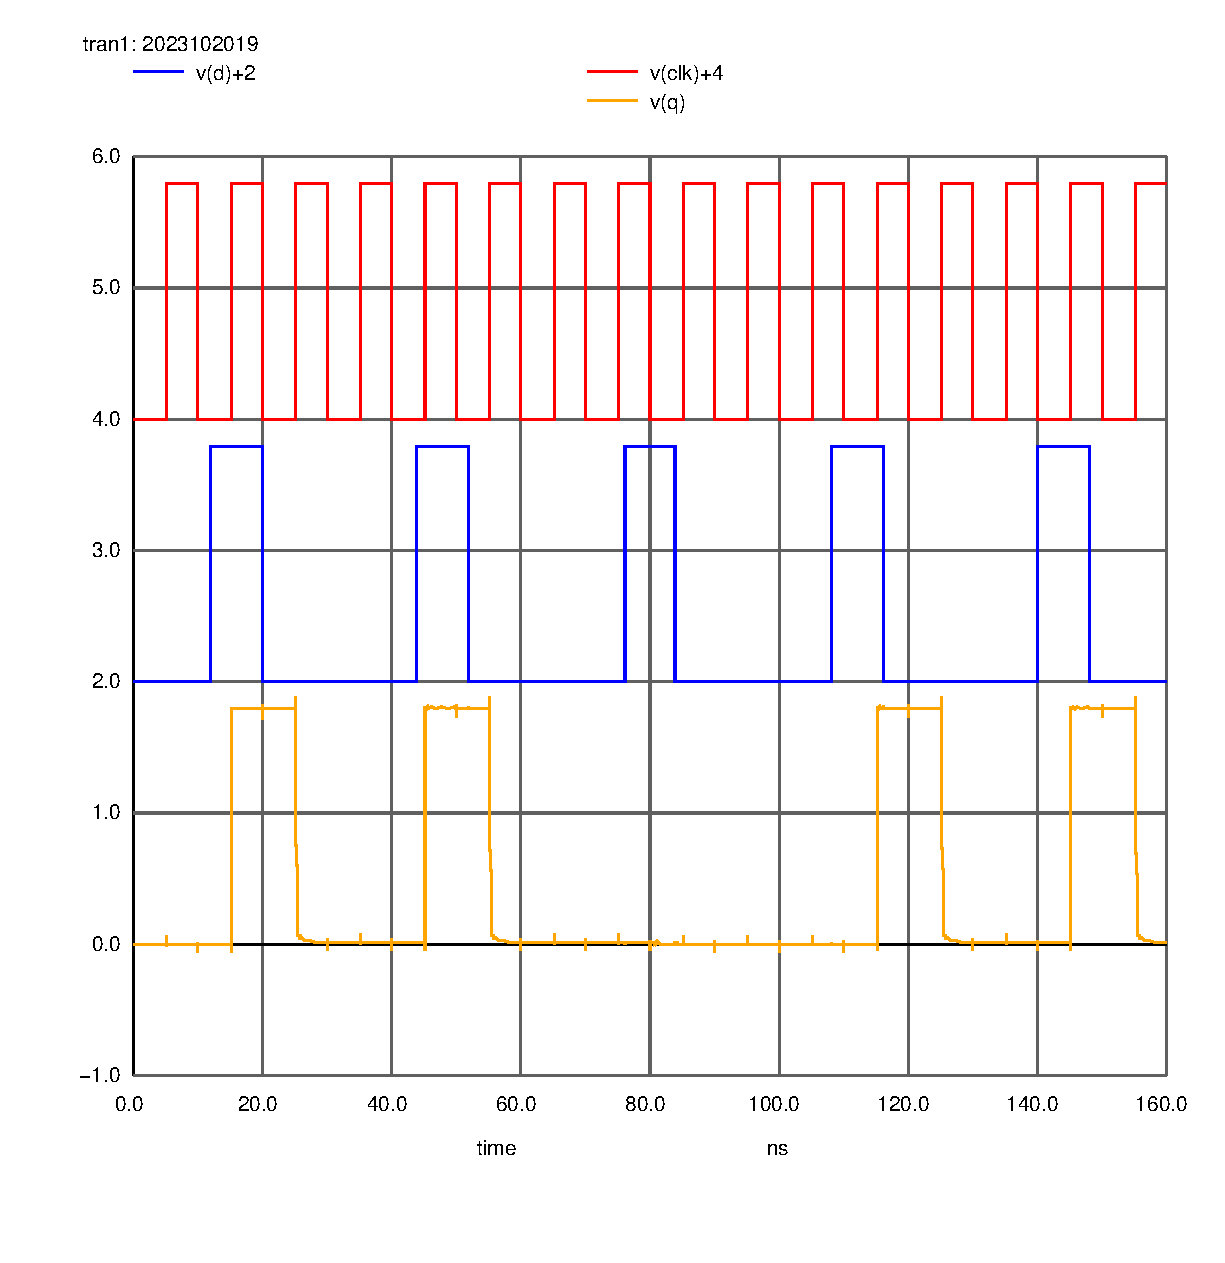
\includegraphics[width=0.48\textwidth]{images/d_ff_optimized_tran.eps}
    \caption{NGSPICE Plot of Optimized D Flip Flop}
\end{figure}

\subsection{Full Circuit}

\subsubsection{CMOS Implementation}

\begin{figure}[H]
    \centering
    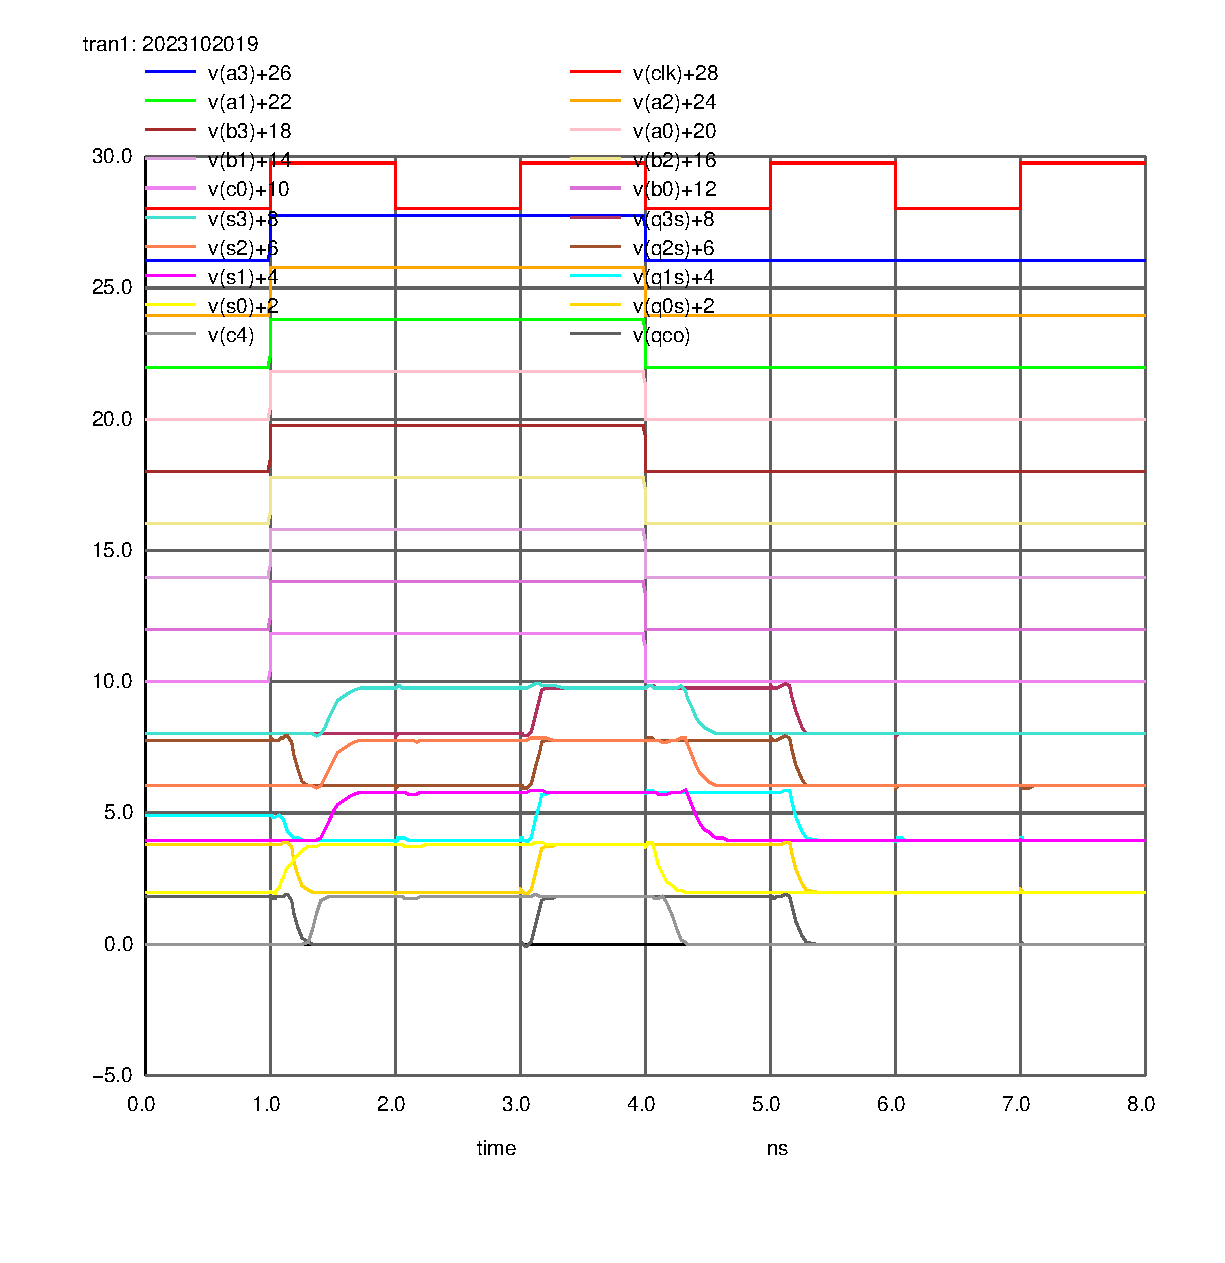
\includegraphics[width=0.48\textwidth]{images/full_cmos_tran.eps}
    \caption{NGSPICE Plot of CMOS Circuit}
\end{figure}

\subsubsection{Optimized Implementation}

\begin{figure}[H]
    \centering
    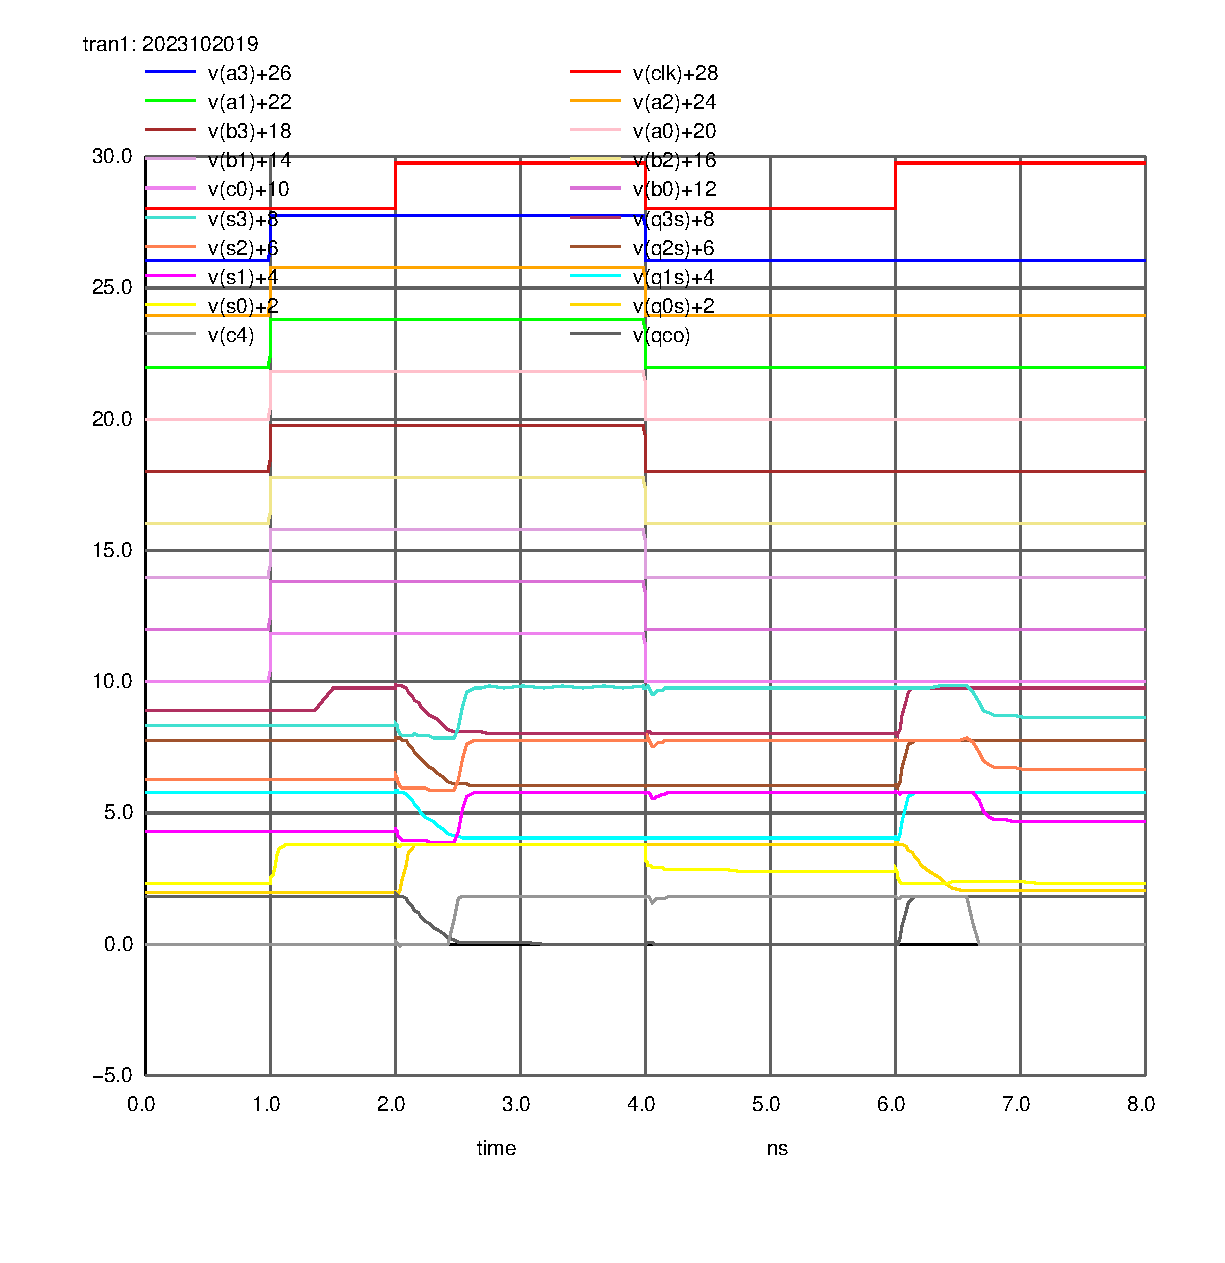
\includegraphics[width=0.48\textwidth]{images/full_optimized_tran.eps}
    \caption{NGSPICE Plot of Optimized Circuit}
\end{figure}

\section{MAGIC Layout}

\subsection{Inverter}

\begin{figure}[H]
    \centering
    \includegraphics[width=0.48\textwidth]{images/inv_cmos_layout.png}
    \caption{MAGIC Layout of CMOS Inverter}
\end{figure}

\subsection{NAND Gate}

\begin{figure}[H]
    \centering
    \begin{tabular}{cc}
        \begin{subfigure}{0.44\linewidth}
            \centering
            \includegraphics[width=\textwidth]{images/nand_cmos_layout.png}
            \caption{2 Input NAND}
        \end{subfigure} &
        \begin{subfigure}{0.44\linewidth}
            \centering
            \includegraphics[width=\textwidth]{images/nand_3_cmos_layout.png}
            \caption{3 Input NAND}
        \end{subfigure} \\
        \begin{subfigure}{0.44\linewidth}
            \centering
            \includegraphics[width=\textwidth]{images/nand_4_cmos_layout.png}
            \caption{4 Input NAND}
        \end{subfigure} &
        \begin{subfigure}{0.44\linewidth}
            \centering
            \includegraphics[width=\textwidth]{images/nand_5_cmos_layout.png}
            \caption{5 Input NAND}
        \end{subfigure}
    \end{tabular}
    \caption{MAGIC Layout of NAND Gates}
\end{figure}

\subsection{NOR Gate}

\begin{figure}[H]
    \centering
    \begin{tabular}{cc}
        \begin{subfigure}{0.44\linewidth}
            \centering
            \includegraphics[width=\textwidth]{images/nor_cmos_layout.png}
            \caption{2 Input NOR}
        \end{subfigure} &
        \begin{subfigure}{0.44\linewidth}
            \centering
            \includegraphics[width=\textwidth]{images/nor_3_cmos_layout.png}
            \caption{3 Input NOR}
        \end{subfigure} \\
        \begin{subfigure}{0.44\linewidth}
            \centering
            \includegraphics[width=\textwidth]{images/nor_4_cmos_layout.png}
            \caption{4 Input NOR}
        \end{subfigure} &
        \begin{subfigure}{0.44\linewidth}
            \centering
            \includegraphics[width=\textwidth]{images/nor_5_cmos_layout.png}
            \caption{5 Input NOR}
        \end{subfigure}
    \end{tabular}
    \caption{MAGIC Layout of NOR Gates}
\end{figure}

\subsection{XOR Gate}

\begin{figure}[H]
    \centering
    \includegraphics[width=0.48\textwidth]{images/xor_optimized_layout.png}
    \caption{MAGIC Layout of XOR Gate}
\end{figure}

\subsection{Propagate/Generate Generator}

\begin{figure}[H]
    \centering
    \includegraphics[width=0.48\textwidth]{images/pg_gen_optimized_layout.png}
    \caption{MAGIC Layout of Propagate/Generate Generator}
\end{figure}

\subsection{Carry Look Ahead Generator}

\begin{figure}[H]
    \centering
    \includegraphics[width=0.48\textwidth]{images/cla_gen_cmos_layout.png}
    \caption{MAGIC Layout of Carry Look Ahead Generator}
\end{figure}

\subsection{Sum Generator}

\begin{figure}[H]
    \centering
    \includegraphics[width=0.48\textwidth]{images/sum_gen_optimized_layout.png}
    \caption{MAGIC Layout of Sum Generator}
\end{figure}

\subsection{D Flop Flop}

\subsubsection{CMOS Implementation}

\begin{figure}[H]
    \centering
    \includegraphics[width=0.48\textwidth]{images/d_ff_cmos_layout.png}
    \caption{MAGIC Layout of CMOS D Flip Flop}
\end{figure}

\subsubsection{Optimized Implementation}

\begin{figure}[H]
    \centering
    \includegraphics[width=0.48\textwidth]{images/d_ff_optimized_layout.png}
    \caption{MAGIC Layout of Optimized D Flip Flop}
\end{figure}


\subsection{Full Circuit}

\begin{figure*}[t]
    \centering
    \includegraphics[width=1\textwidth]{images/full_optimized_layout.png}
    \caption{MAGIC Layout of Full Circuit}
\end{figure*}

\section{Post Layout Simulation}

\subsection{Inverter}

\begin{figure}[H]
    \centering
    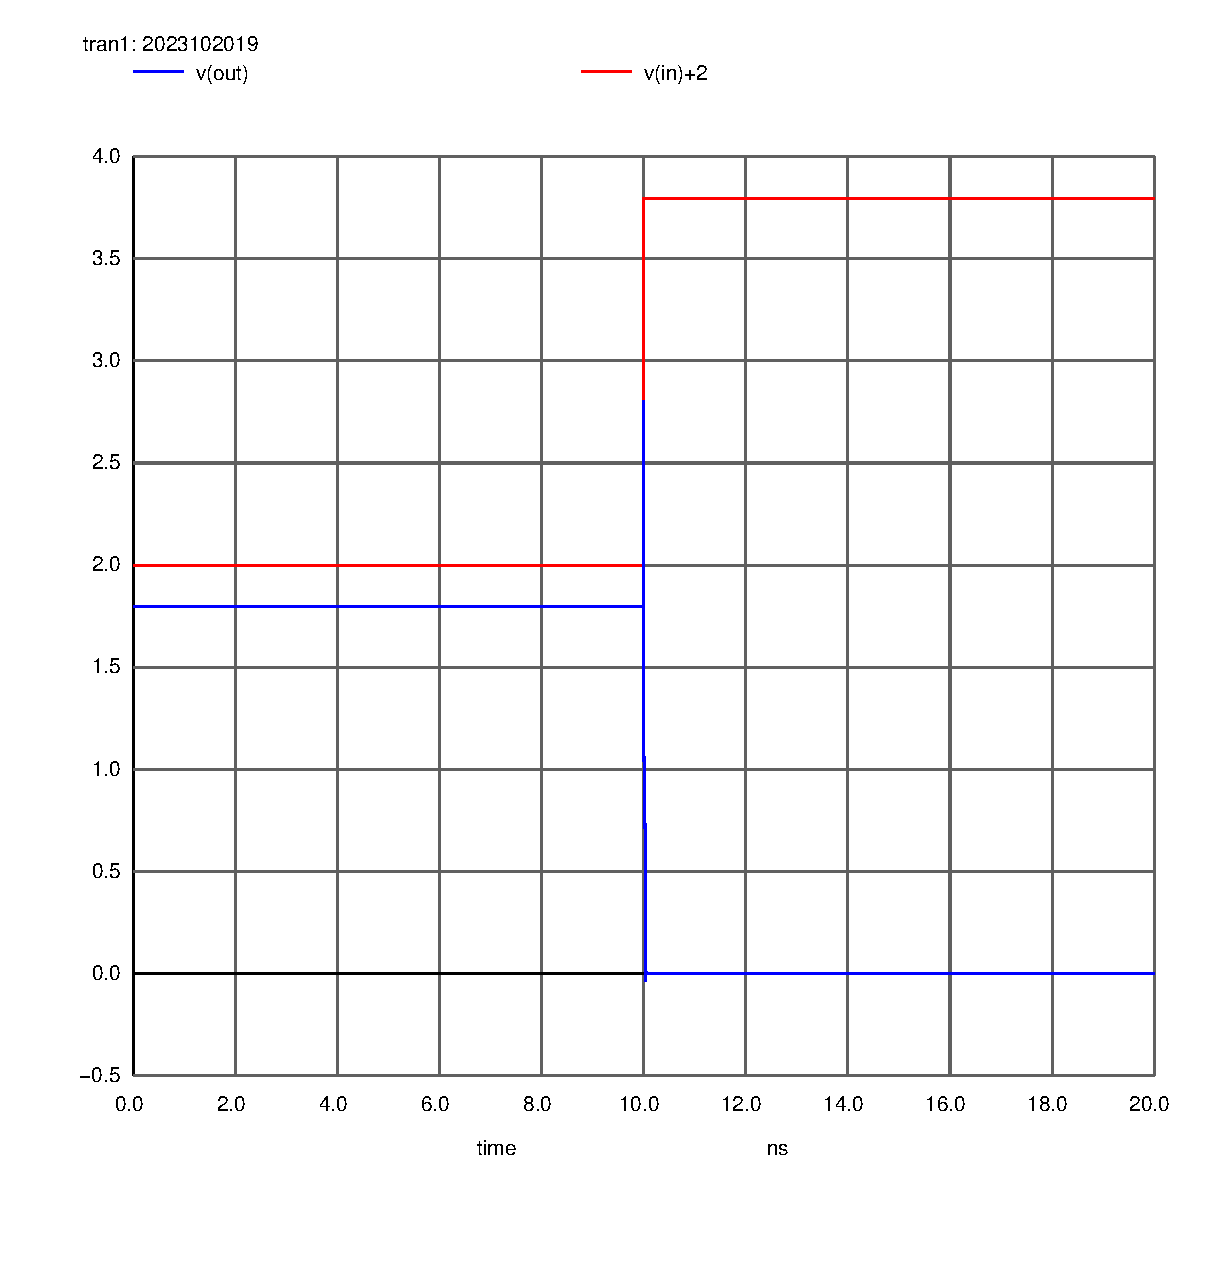
\includegraphics[width=0.48\textwidth]{images/inv_cmos_post_tran.eps}
    \caption{Post Layout NGSPICE Plot of Inverter}
\end{figure}

\subsection{NAND Gate}

\begin{figure}[H]
    \centering
    \begin{tabular}{cc}
        \begin{subfigure}{0.44\linewidth}
            \centering
            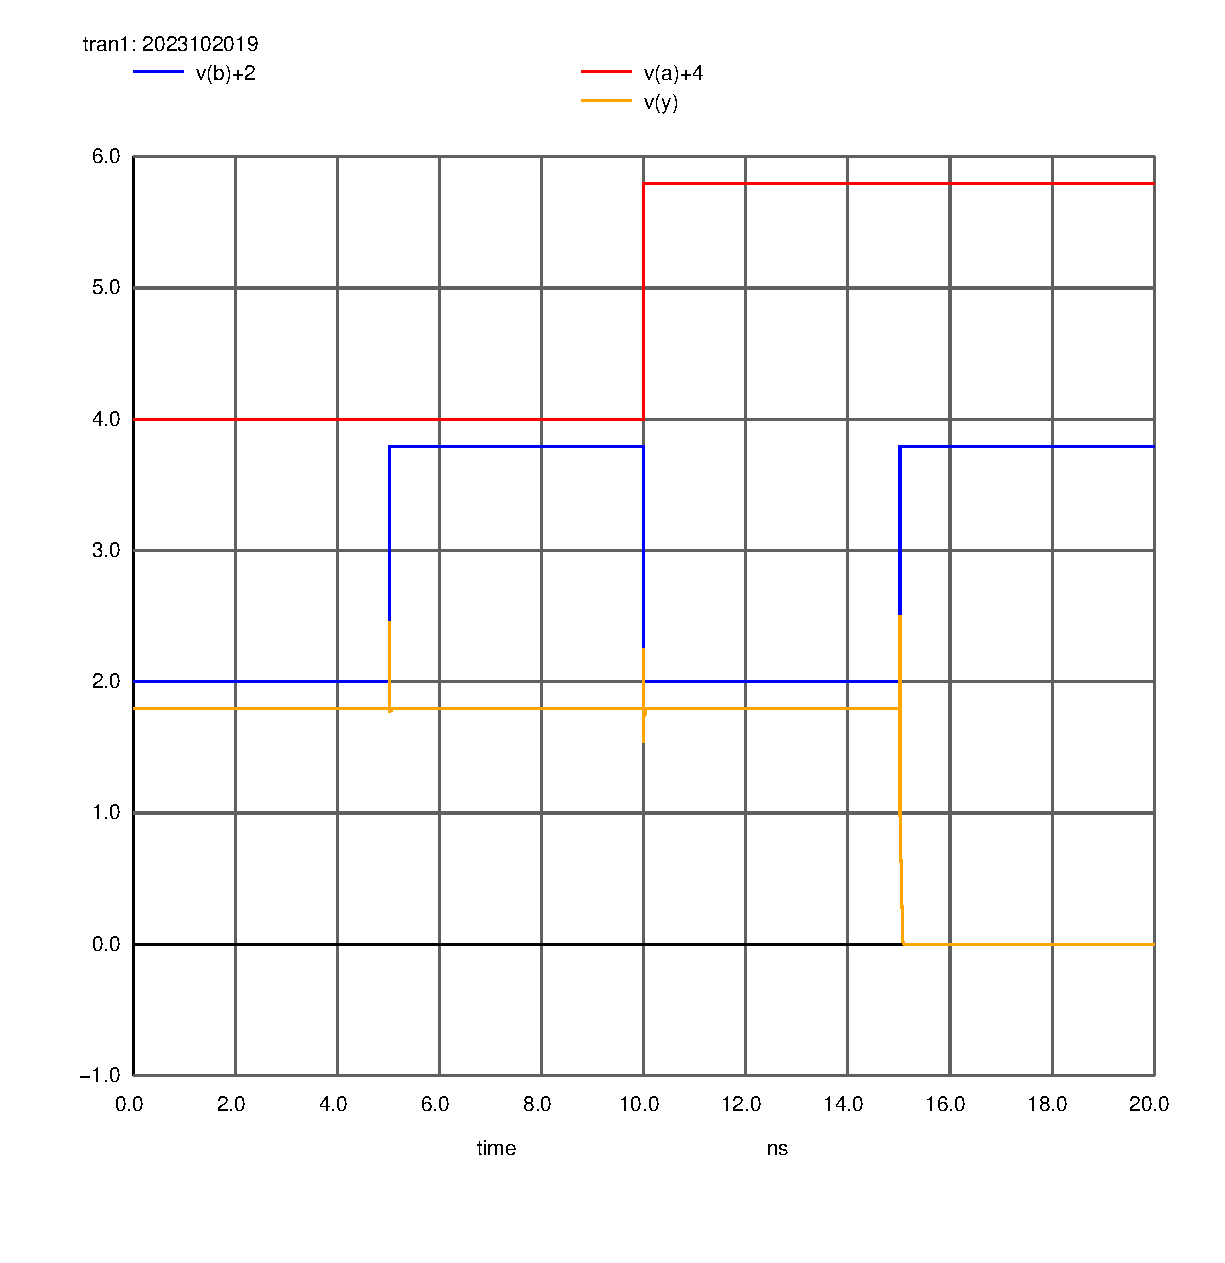
\includegraphics[width=\textwidth]{images/nand_cmos_post_tran.eps}
            \caption{2 Input NAND}
        \end{subfigure} &
        \begin{subfigure}{0.44\linewidth}
            \centering
            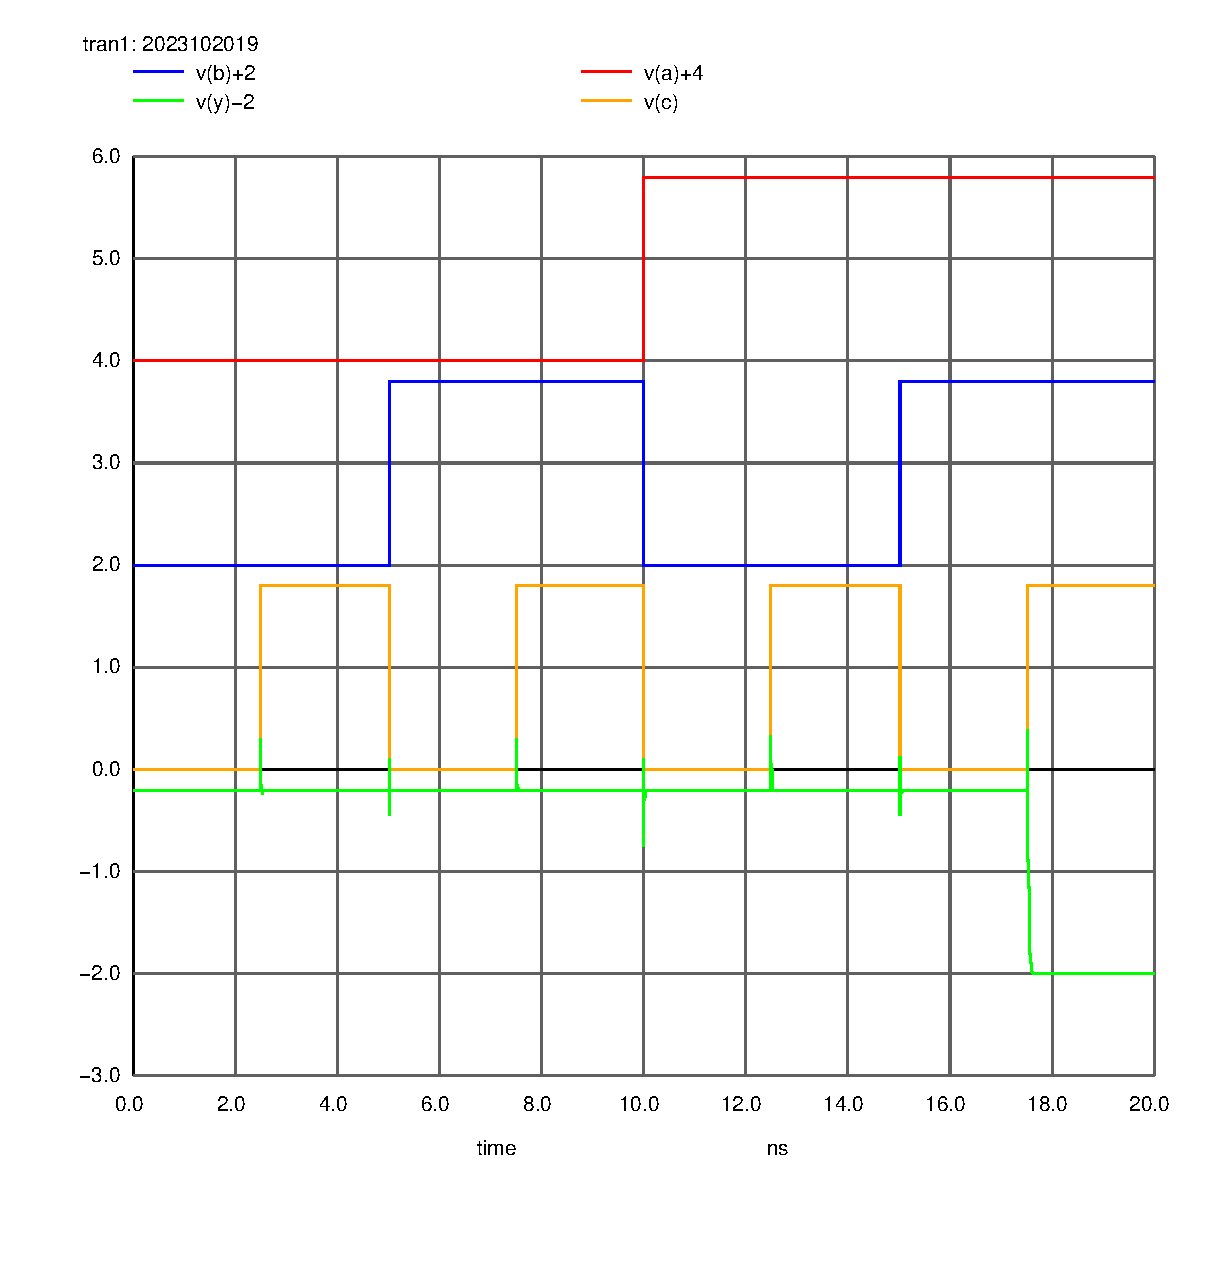
\includegraphics[width=\textwidth]{images/nand_3_cmos_post_tran.eps}
            \caption{3 Input NAND}
        \end{subfigure} \\
        \begin{subfigure}{0.44\linewidth}
            \centering
            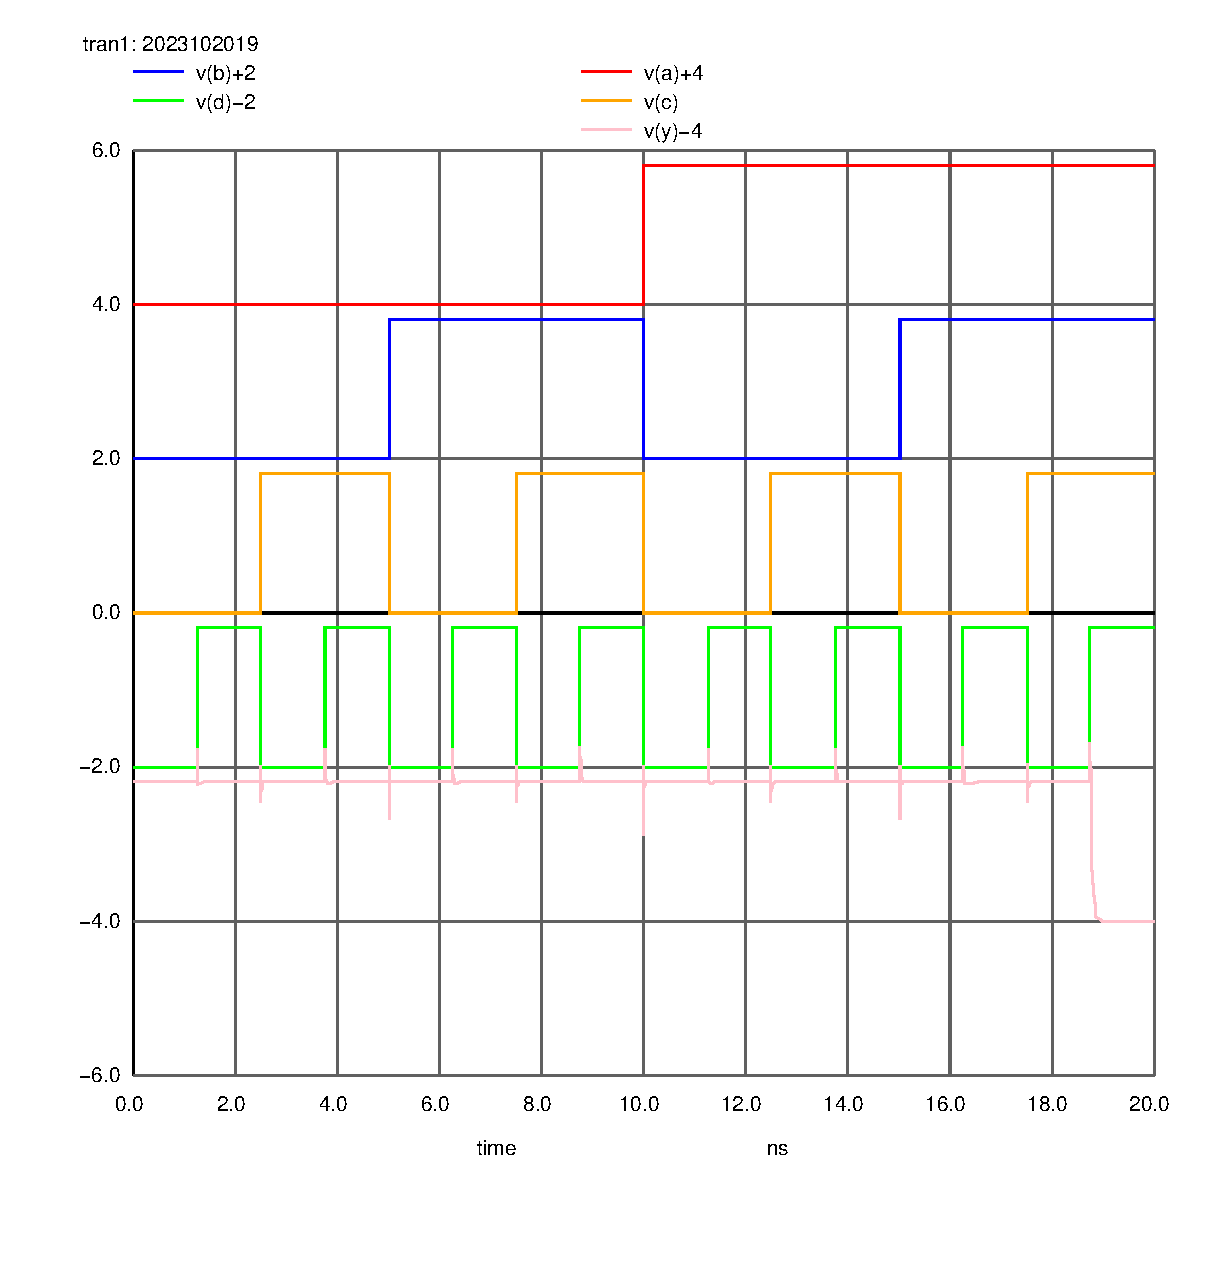
\includegraphics[width=\textwidth]{images/nand_4_cmos_post_tran.eps}
            \caption{4 Input NAND}
        \end{subfigure} &
        \begin{subfigure}{0.44\linewidth}
            \centering
            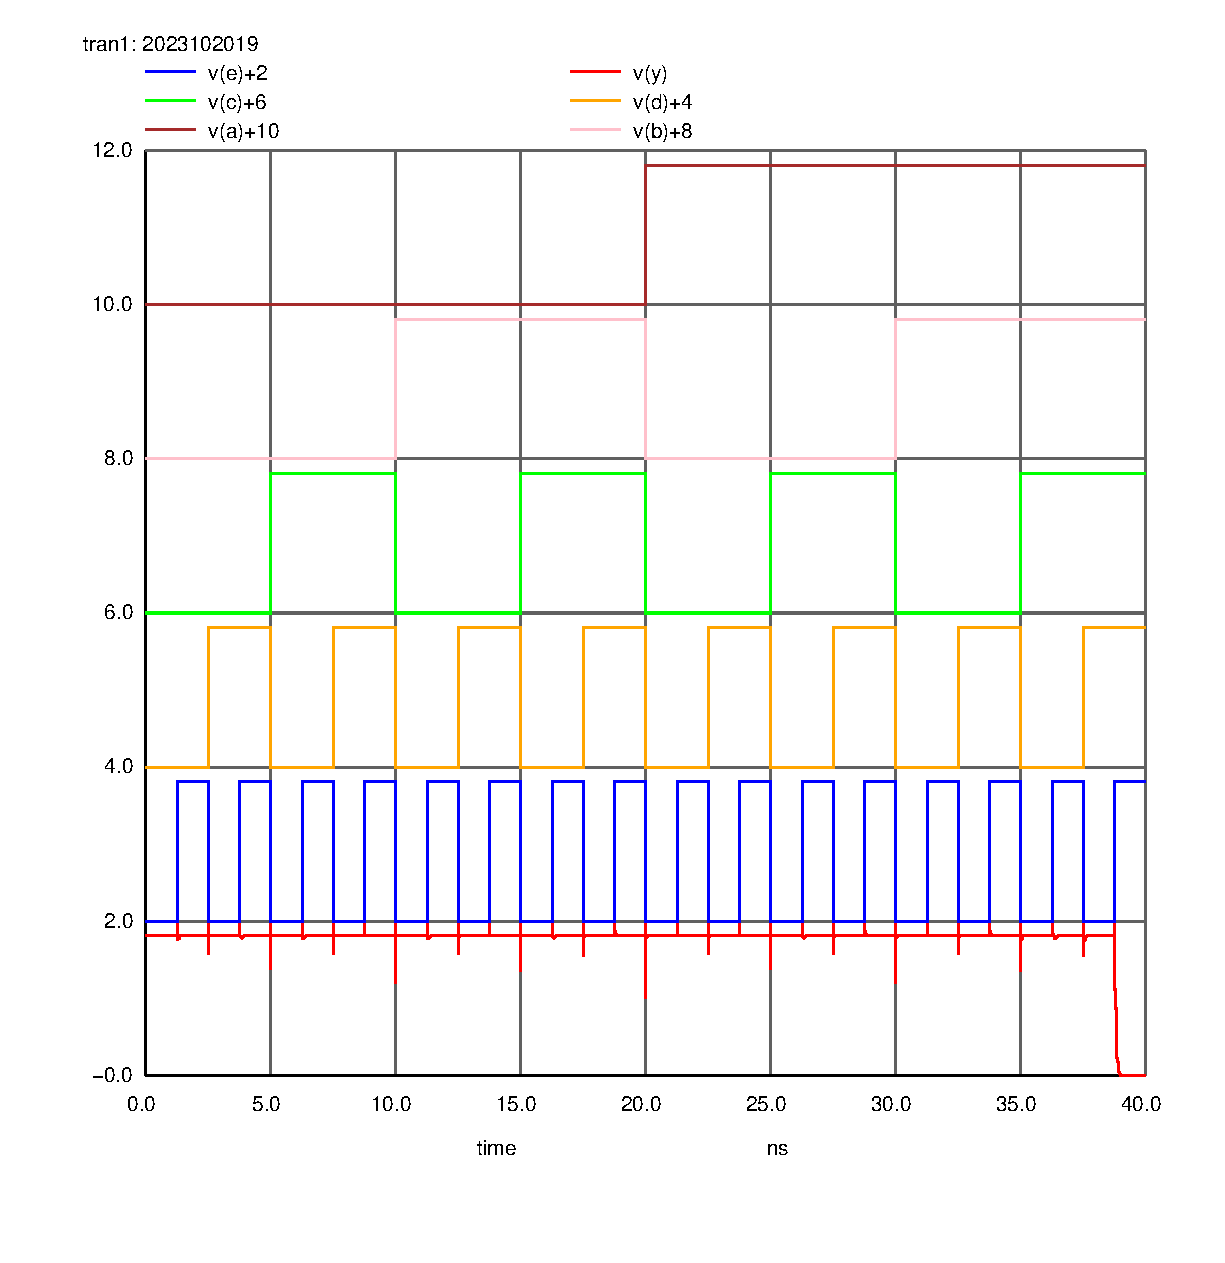
\includegraphics[width=\textwidth]{images/nand_5_cmos_post_tran.eps}
            \caption{5 Input NAND}
        \end{subfigure}
    \end{tabular}
    \caption{Post Layout NGSPICE Plot of NAND Gates}
\end{figure}

\subsection{NOR Gate}

\begin{figure}[H]
    \centering
    \begin{tabular}{cc}
        \begin{subfigure}{0.44\linewidth}
            \centering
            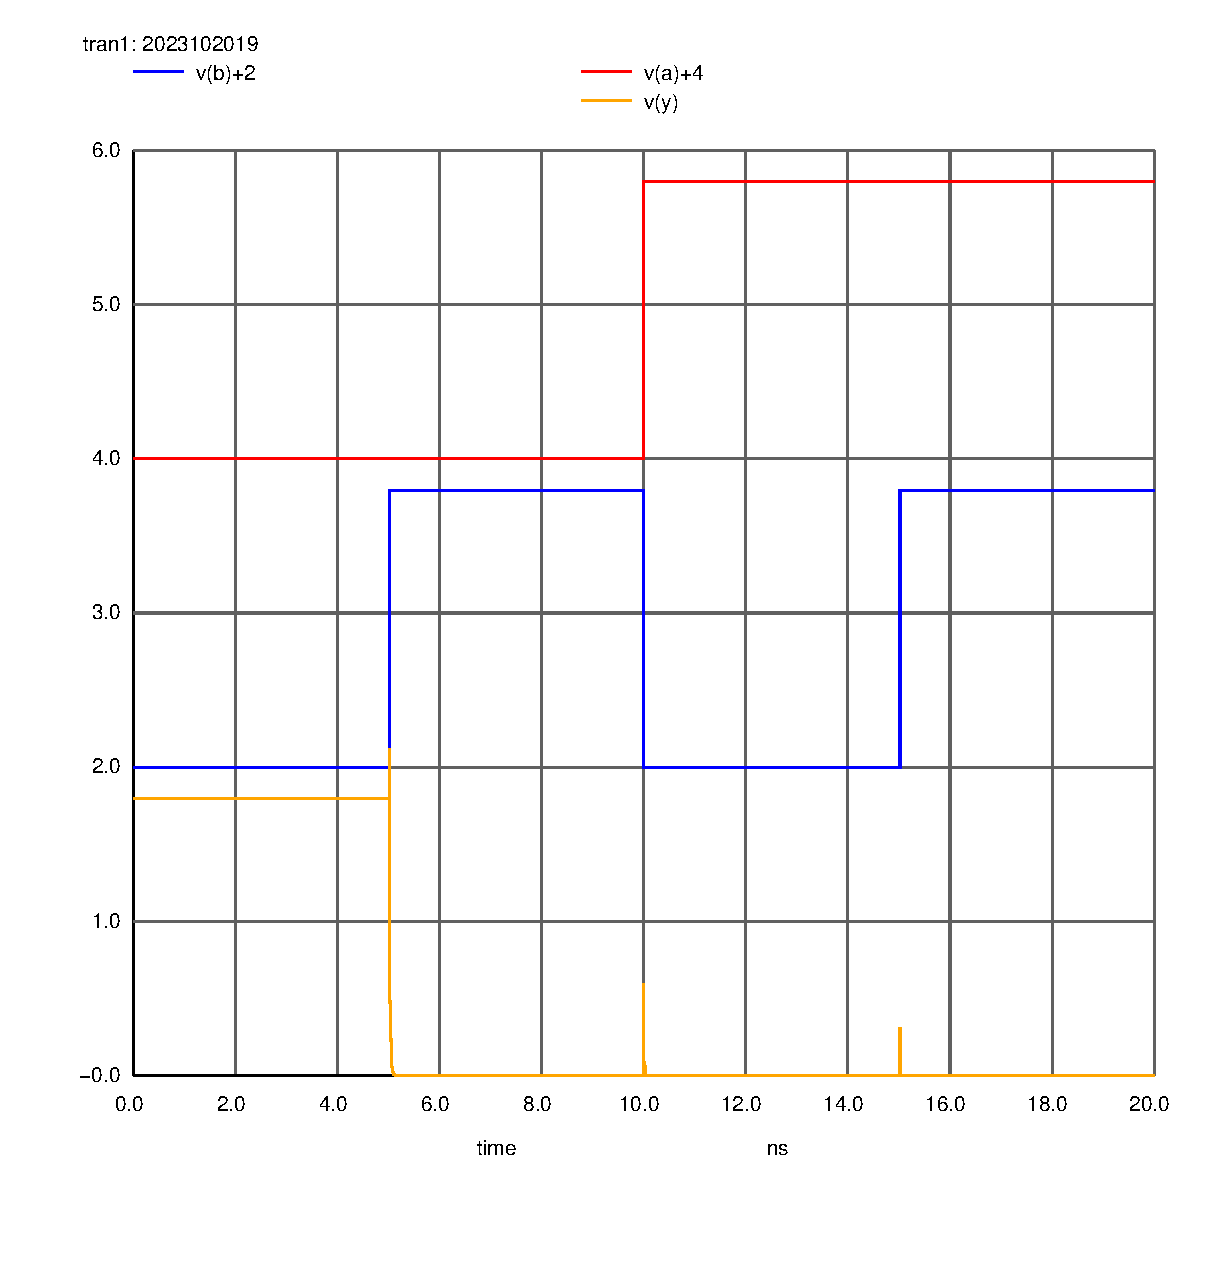
\includegraphics[width=\textwidth]{images/nor_cmos_post_tran.eps}
            \caption{2 Input NOR}
        \end{subfigure} &
        \begin{subfigure}{0.44\linewidth}
            \centering
            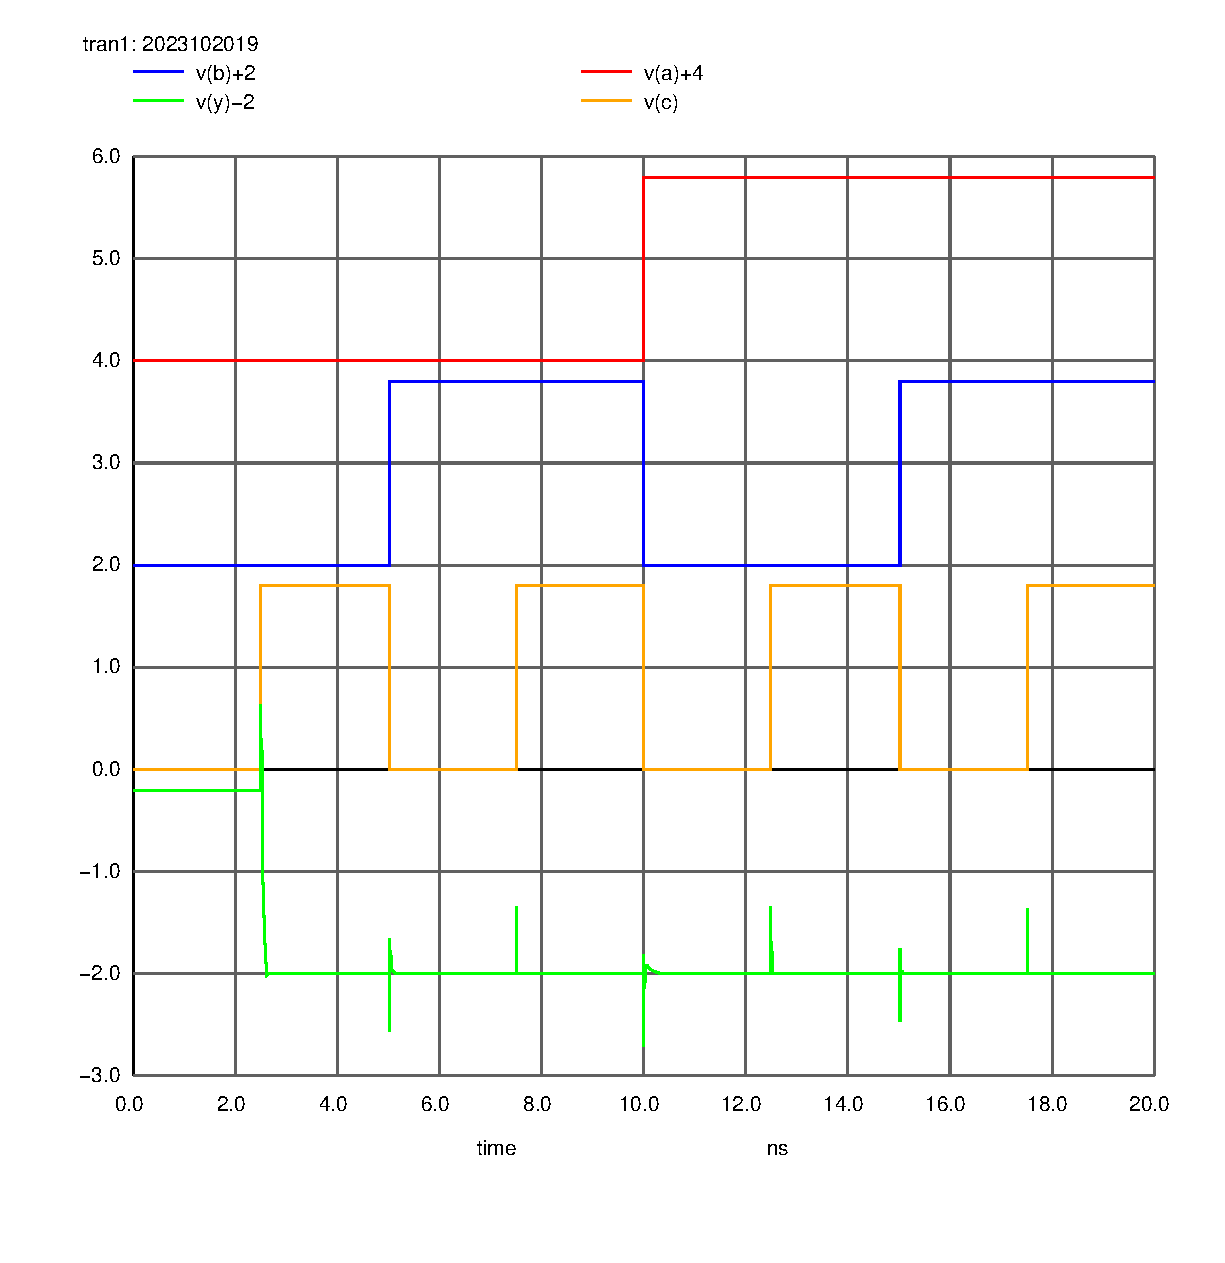
\includegraphics[width=\textwidth]{images/nor_3_cmos_post_tran.eps}
            \caption{3 Input NOR}
        \end{subfigure} \\
        \begin{subfigure}{0.44\linewidth}
            \centering
            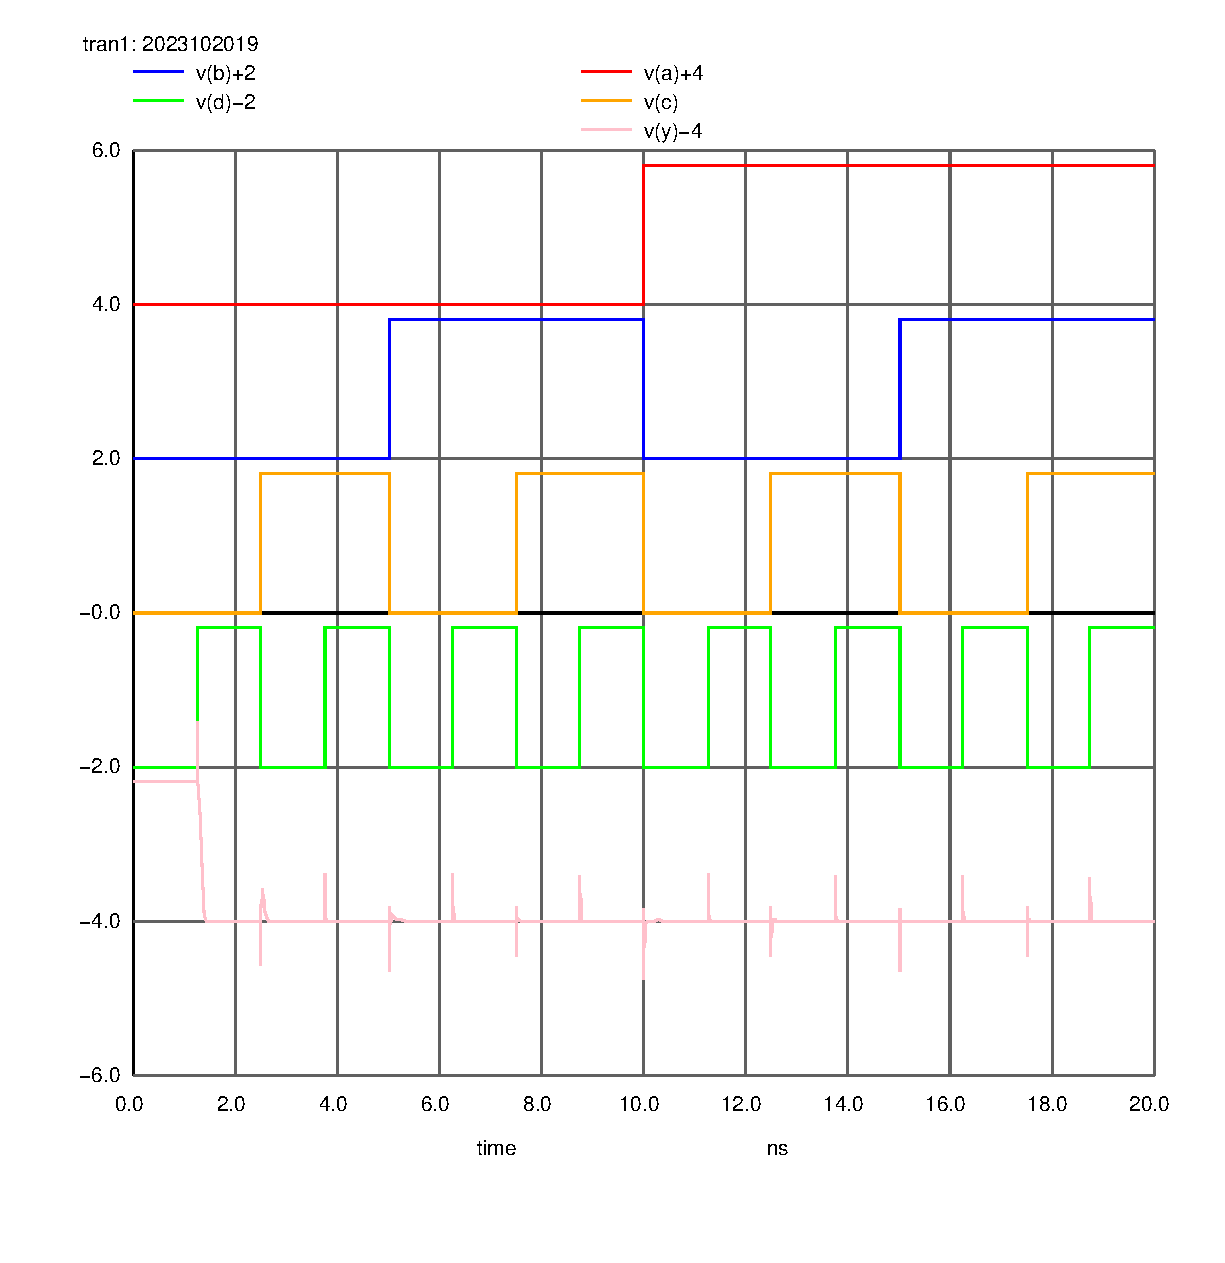
\includegraphics[width=\textwidth]{images/nor_4_cmos_post_tran.eps}
            \caption{4 Input NOR}
        \end{subfigure} &
        \begin{subfigure}{0.44\linewidth}
            \centering
            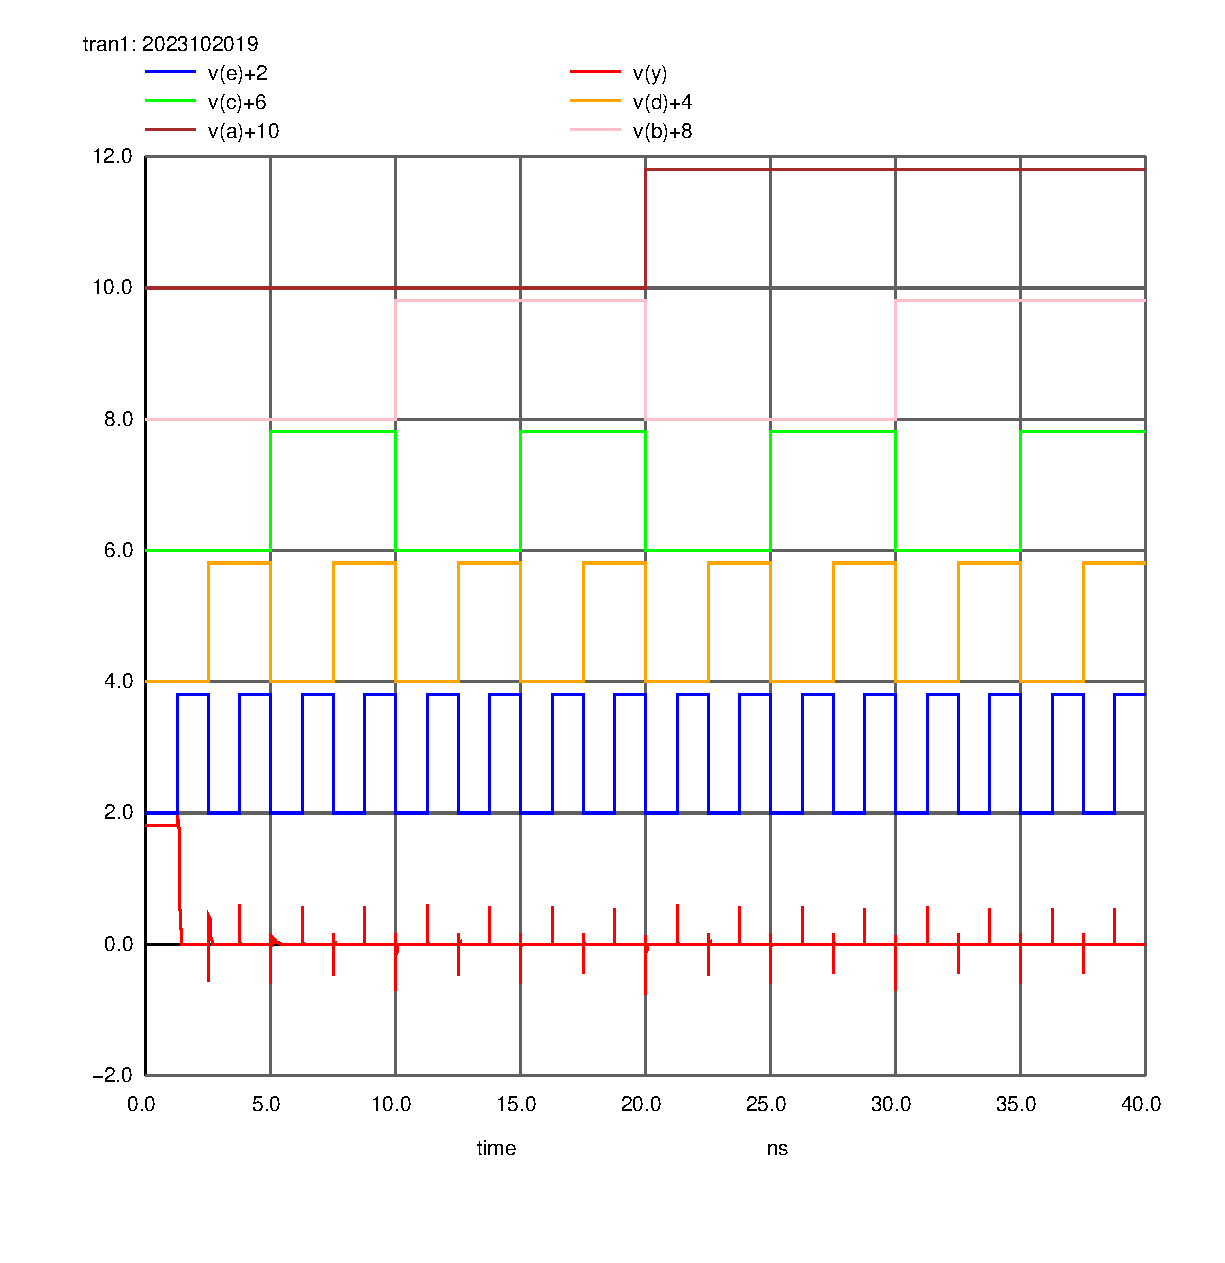
\includegraphics[width=\textwidth]{images/nor_5_cmos_post_tran.eps}
            \caption{5 Input NOR}
        \end{subfigure}
    \end{tabular}
    \caption{Post Layout NGSPICE Plot of NOR Gates}
\end{figure}

\subsection{XOR Gate}

\begin{figure}[H]
    \centering
    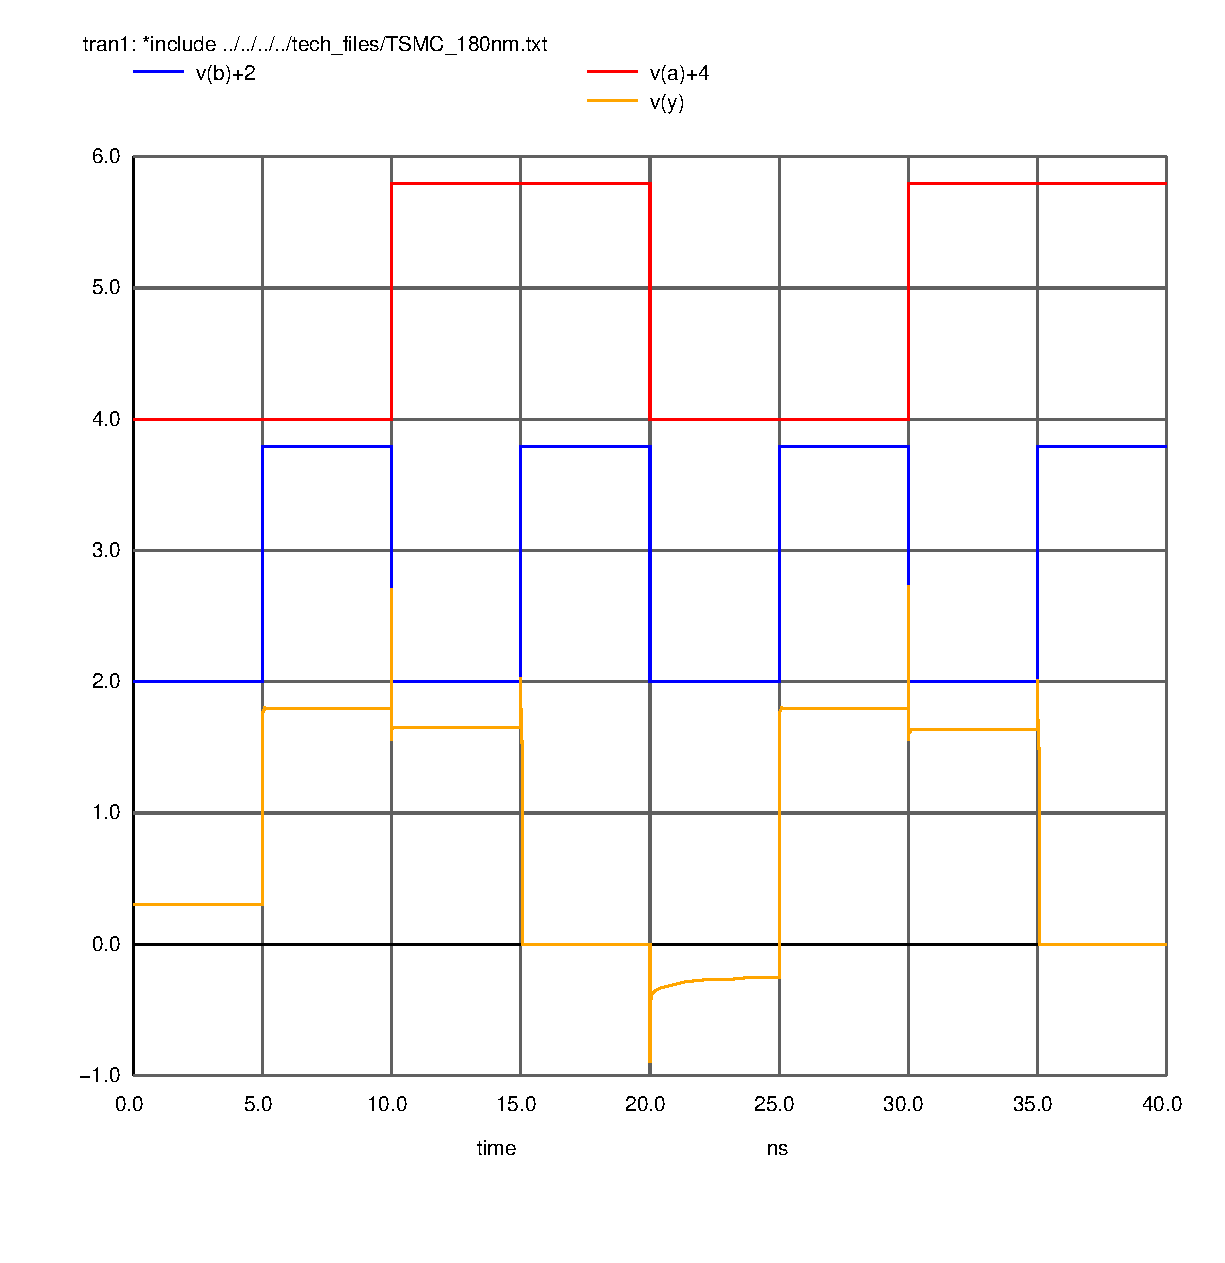
\includegraphics[width=0.48\textwidth]{images/xor_optimized_post_tran.eps}
    \caption{Post Layout NGSPICE Plot of XOR Gate}
\end{figure}

\subsection{D Flop Flop}

\begin{figure}[H]
    \centering
    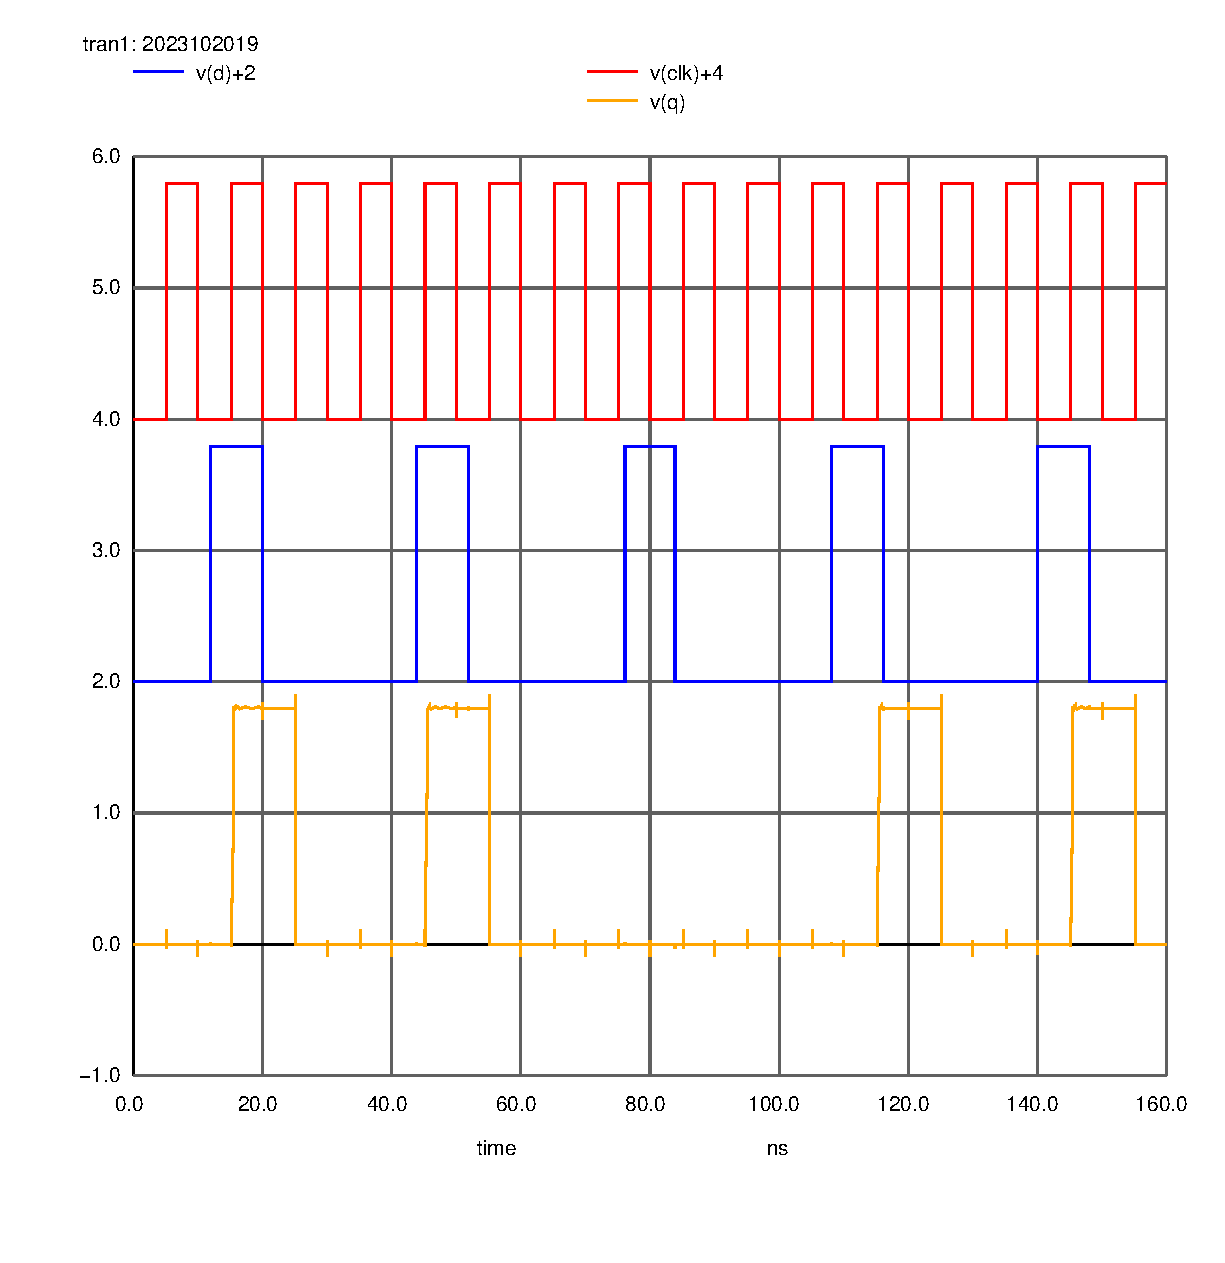
\includegraphics[width=0.48\textwidth]{images/d_ff_optimized_post_tran.eps}
    \caption{Post Layout NGSPICE Plot of D Flip Flop}
\end{figure}

\subsection{Full Circuit (with Load Inverters)}

\begin{figure}[H]
    \centering
    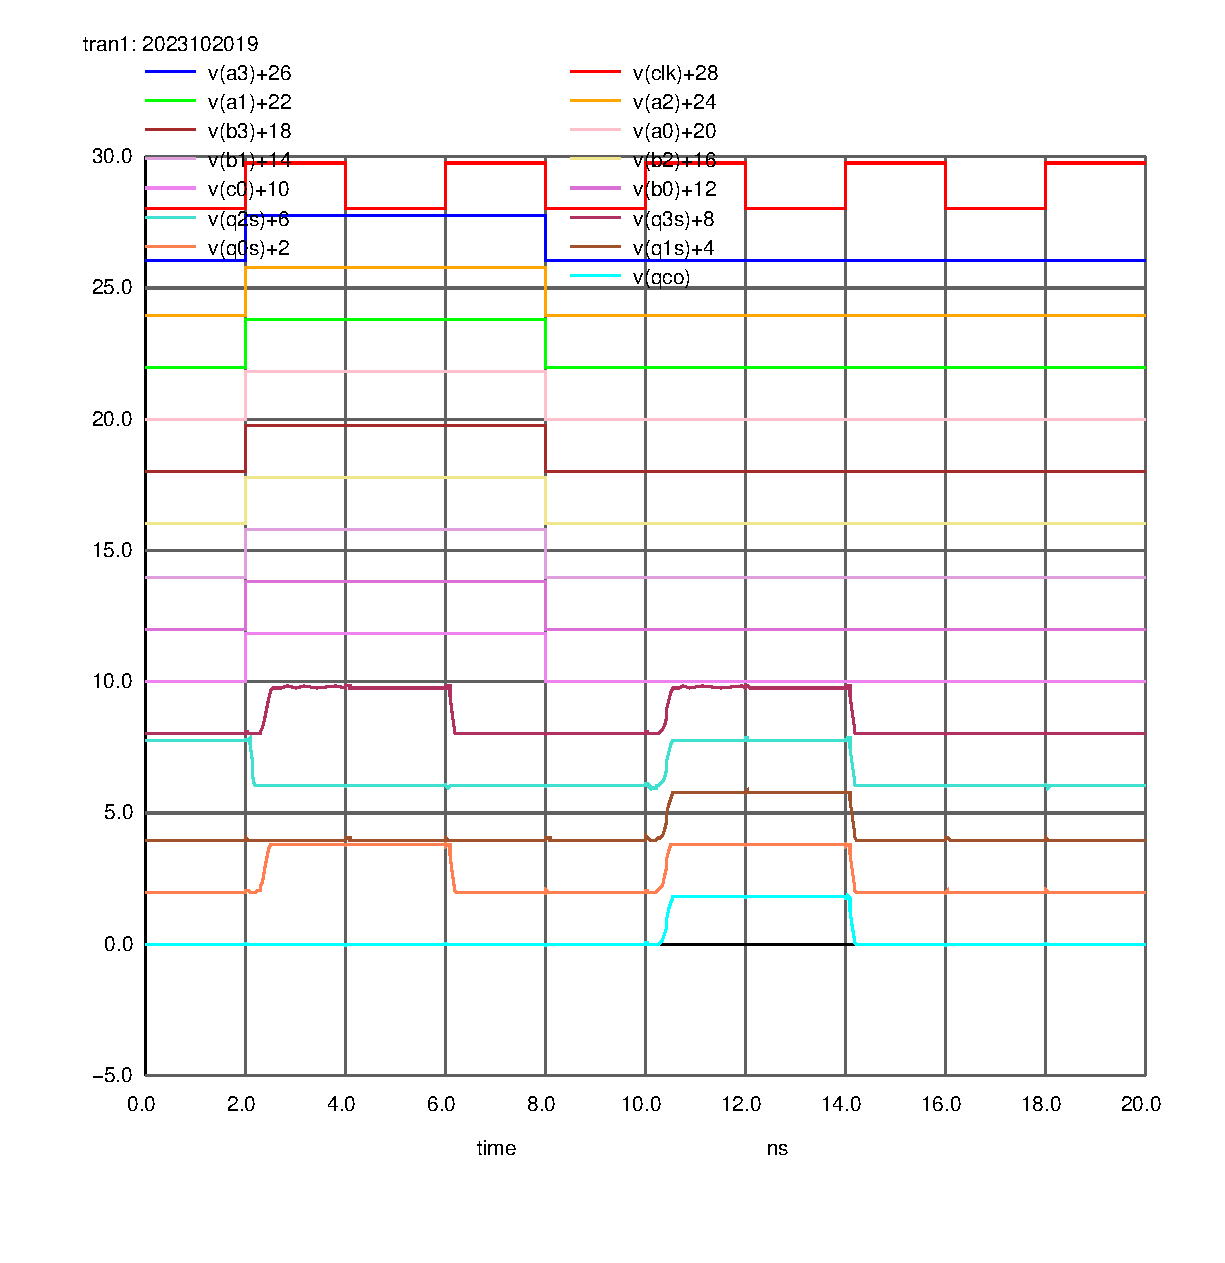
\includegraphics[width=0.48\textwidth]{images/full_optimized_load_post_tran.eps}
    \caption{Post Layout NGSPICE Plot of Full Circuit}
\end{figure}

\section{FPGA Simulation}

\subsection{On Board LEDs}

\begin{figure}[H]
    \centering
    \begin{subfigure}{0.48\textwidth}
        \includegraphics[width=\linewidth]{images/fpga_1.png}
        \caption{1111 + 1111 + 0 = 11110}
    \end{subfigure}
    \hfill
    \begin{subfigure}{0.48\textwidth}
        \includegraphics[width=\linewidth]{images/fpga_2.png}
        \caption{1111 + 1111 + 1 = 11111}
    \end{subfigure}
    \hfill
    \begin{subfigure}{0.48\textwidth}
        \includegraphics[width=\linewidth]{images/fpga_3.png}
        \caption{1011 + 1001 + 1 = 10101}
    \end{subfigure}
    
    \caption{FPGA Simulation}
    \label{fig:main}
\end{figure}

\subsection{Waveform Visualization}

\begin{figure}[H]
    \centering
    \includegraphics[width=0.48\textwidth]{images/fpga_waveform.png}
    \caption{Viewing Waveform of FPGA Simulation}
\end{figure}

\section*{Acknowledgment}


\begin{thebibliography}{00}
\bibitem{b1} 
\end{thebibliography}

\end{document}


